% -*- TeX:SI -*-
% slovene sub-mode for spell check
% ----------------------------------------------------------------------
%  Predloga za obliko in navodila za pisanje diplomskih nalog v LaTex-u

%  Univerza v Ljubljani, Fakulteta za elektrotehniko

%  zbral in uredil Roman Kamnik, junij 2013

% ----------------------------------------------------------------------

\documentclass[a4paper,twoside,openright,12pt]{book}
\usepackage[a-1b]{pdfx}   % for PDF/A-1b
% \usepackage[x-1a]{pdfx}  % for PDF/X-1a

\usepackage[utf8]{inputenc}  %Kodna stran za Windows okolje, za linux je kodna stran latin2
%\usepackage[T1]{fontenc}
\usepackage[slovene]{babel}    % pravila za slovensko deljenje besed
\usepackage[pdftex]{UNI-LJ-FE-Diploma} %Stil za diplome na Fakulteti za elektrotehniko (za pdfTeX v MkiTex)
%\usepackage[pctex]{UNI-LJ-FE-Diploma} %Stil za diplome na Fakulteti za elektrotehniko  (za pcTex)



% Not working \usepackage{natbib} % for \citeathor \citeyear
%%%%%%%%%%%%%%%%%%%%%%%%
% MATEMATIKA IN FIZIKA %
%%%%%%%%%%%%%%%%%%%%%%%%
% za matematiko
\usepackage{amsmath, amsfonts, xfrac, amssymb, mathrsfs, amsthm, bm}
% za enote
% \si{enota}
% \SI{cifra}{enota}
% \num{cifra}
% \ang{kot}
\usepackage{siunitx}
% Declare new unit
\DeclareSIUnit{\cal}{cal}
\DeclareSIUnit{\kcal}{\kilo\cal}
\DeclareSIUnit{\joul}{\J}
\DeclareSIUnit{\kjoul}{\kJ}
\DeclareSIUnit{\min}{\minute}
\sisetup{output-decimal-marker = {,}}
\sisetup{separate-uncertainty=true,multi-part-units=single}
\sisetup{range-phrase = --}
%\sisetup{per-mode=reciprocal}
%\sisetup{group-separator = {.}}
% za uporabljanje decimalne vejice in ne pike
% pises decimalno piko, vendar ti zgenerira kot decimalno vejico
% to zato, da ko uporabljas vejico imas za vejico avtomatsko presledek
%\DeclareMathSymbol{.}{\mathord}{letters}{"3B}
% lahko bi uporabil tudi novo komando
\newcommand{\vejica}{{,}}
% lahko pa uporabljas \num{stevilka}, iz paketa siunitx

% za (1-3) pri enačbah
%\usepackage{cleveref}

%%%%%%%%%%%%%%%%%%%%%%%%%%%%%%
% TABELE IN SLIKE NASTEVANJE %
%%%%%%%%%%%%%%%%%%%%%%%%%%%%%%
%
% for adding tables that can span across multiple columns
\usepackage{xtab}
% za uporabo toprule bottomrule midrule za boljse tabele
\usepackage{booktabs} 
\usepackage[]{multirow}
% za align-annje na decimalni vejici
\usepackage{dcolumn}
% USAGE: ...\begin{tabular}{l r c D{separator in tex file}{ separator in output}{decimal places}}
% ovveride in heading with \multicolumn{1}{..}{..}

% za tabele katerim dolocimo širino in X specifier -> ta naredi stolpec tako
% dolg, da bo tabela zavzela določeno širino.
\usepackage{tabularx}
% ovveride in heading with \multicolumn{1}{..}{..}
\usepackage{etoolbox}
%\robustify\bfseries
\usepackage{longtable}

% za dodajanje slik
\usepackage{graphicx}
\graphicspath{{./Slike/}}
\usepackage{epstopdf}
\usepackage{caption}
\usepackage{subcaption}

% Za dodajanje okvirjev okoli slik
\usepackage[export]{adjustbox}
% USAGE: 
% \includegraphics[<other options>, frame]{image}
% or
% \includegraphics[<other options>, fbox]{image}

% za tikz slikce
\usepackage{pgfplots}
\pgfplotsset{compat=1.12}
\usepgfplotslibrary{polar}
\pgfplotsset{plot style/.style={axis x line=middle, axis y line=
middle, xlabel={$x$}, ylabel={$y$}, axis equal }}

\pgfplotsset{polar plot style/.style = {
xticklabels={,,
$\frac{\pi}{6}$, $\frac{\pi}{3}$, $\frac{\pi}{2}$, $\frac{2\pi}{3}$,
$\frac{5\pi}{6}$, $\pi$, $\frac{7\pi}{6}$, $\frac{4\pi}{3}$,
$\frac{3\pi}{2}$, $\frac{5\pi}{3}$,$\frac{11\pi}{6}$,}, thick
}}

\pgfplotsset{hoof plot style/.style = {
polar plot style,
xtick={0,30,60,90,120,150,180,210,240,270,300,330},
xticklabels={$3$, $4$, $5$, $6$, $5$, $4$, $3$, $2$, $1$,, $1$, $2$}
}}

\usepackage{circuitikz, tikz, tikz-3dplot}
\usetikzlibrary{arrows, shapes, positioning, intersections, calc, shadings}
\usetikzlibrary{3d}
\newcommand{\blokec}[2]{node[draw, text centered, minimum width=4cm, minimum height=1cm, rounded corners, text width= 3cm, scale=1](#1){#2}}
    
\tikzset{dash/.style = {dashed, draw=black!50}}
\tikzset{dot/.style = {dotted, draw=black!50}}
\tikzset{base-axis/.style = {very thick}}
\tikzset{axis/.style = {base-axis, ->, >=stealth}}
\tikzset{plane/.style = {
	fill=teal!20, opacity=0.8,
    draw=teal!50!black!50,
    solid, thick
    }}
      
\tikzset{vec/.style = {->, >=stealth, solid, thick}}

\tikzset{velocity/.style = { vec, draw=orange!50!black!90}}


\tikzset{rect/.style = {
  rectangle,
  very thick, solid, rounded corners=1mm,
  top color=white,
  text centered, align=center,
  scale = 0.7
  }}
  \tikzset{title/.style = {
  % Rectangle:
  rect,
  draw=red!50!black!50,
  bottom color=red!50!black!20,
  % Text:
  text width = 30mm
  }}
  \tikzset{block/.style = {
  % Rectangle:
  rect,
  draw=black!50,
  bottom color=black!20
  % Text
  }}
  \tikzset{input/.style = {
  % Rectangle:
  block,
  draw=green!50!black!50,
  bottom color=green!50!black!20
  % Text
  }}
  \tikzset{output/.style = {
  % Rectangle:
  block,
  draw=orange!50!black!50,
  bottom color=orange!50!black!20
  % Text
  }}
  \tikzset{background/.style = {
  fill=black!10, 
  rounded corners, 
  draw=black!50, 
  dashed
  }}
  \tikzset{arrow/.style = {
  ->,
  >=stealth,
  shorten >= 1mm,
  shorten <= 1mm,
  very thick,
  draw=black!50,
  line width = 1mm
  }}
  \tikzset{angle/.style={
	fill=#1!20, opacity=0.8,
	draw=#1!50!black!50
	}}
  \tikzset{zxplane/.style={canvas is zx plane at y=#1}}
  \tikzset{yxplane/.style={canvas is yx plane at z=#1}}
  \newcommand{\spherical}[3]{xyz spherical cs:radius=#1,longitude=#3,latitude=#2}
  \newcommand{\cylindrical}[3]{xyz cylindrical cs:radius=#1,z=#3,angle=#2}
  

% za odštevanje pri listih
%\usepackage[start=7]{etaremune}
% za seznam kjer lahko spreminjaš številke
% dodati moraš [label = nekaj]
% če hočeš številke dodaš \arabic*
% če hočeš črke dodaš \alph* ali \Alph*
% če hočeš rimske številke dodaš \roman* ali \Roman*
\usepackage{enumitem}
% za listo v dveh stolpcih
\usepackage{multicol}
% za dodajanje besedila iz drugih datotek
\usepackage{verbatim}
% za urlje 
%\usepackage[unicode, hidelinks]{hyperref}
\usepackage{hyperref}
\hypersetup{hidelinks}
\usepackage{bookmark}




%%%%%%%%%%%%%%%%
% NOVE KOMANDE %
%%%%%%%%%%%%%%%%
\usepackage{xspace} % da latex dojame da mora dat presledke med komandami
\newcommand{\stopinj}{^\circ}
\newcommand{\clips}{\uppercase{clips}\xspace}
\newcommand{\sintaksa}[1]{\xspace``\texttt{#1}''\xspace}
\newcommand{\modd}{\uppercase{modd}\xspace}
\newcommand{\ds}{\uppercase{ds}\xspace}
\newcommand{\bn}{Beier-Neely\xspace}
\newcommand{\opencv}{OpenCV\xspace}
\newcommand{\dlib}{Dlib\xspace}

\newcommand{\vomax}{\ensuremath{VO_{2}max}\xspace}
\newcommand{\vo}{\ensuremath{VO_2}\xspace}

\newcommand{{\T}}{\ensuremath{^{\top}}}
\newcommand{\Mu}{M}
\renewcommand{\Xi}{X}
\newcommand{\norm}[1]{\left\lVert #1 \right\rVert}
\renewcommand{\vec}[1]{{\boldsymbol{#1}}}

\newcommand{\nhoof}{\ensuremath{N_{HOOF}}\xspace}
\newcommand{\nhafa}{\ensuremath{N_{HAFA}}\xspace}
\newcommand{\esvr}{\ensuremath{\epsilon}-SVR\xspace}
\newcommand{\nusvr}{\ensuremath{\nu}-SVR\xspace}
\newcommand{\nurbf}{\ensuremath{\nu}-RBF\xspace}
\newcommand{\nughi}{\ensuremath{\nu}-GHI\xspace}
\newcommand{\emse}{\ensuremath{\overline{e}_{MSE}}\xspace}
\newcommand{\fsv}{\ensuremath{f_{SV}}\xspace}
\newcommand{\numax}{\ensuremath{\nu_{max}}\xspace}
\newcommand{\hrtmax}{\ensuremath{hr_{tmax}}\xspace}

\newcommand{\folder}{./}

\newcommand{\corr}{{CORR}\xspace}
\newcommand{\rmse}{{RMSE}\xspace}
\newcommand{\rae}{{RAE}\xspace}
\newcommand{\rrse}{{RRSE}\xspace}
\newcommand{\nsv}{\fsv}


\newcommand{\boldentry}[3]{%
  \multicolumn{1}{S[table-format=#1.#2,
				  	round-mode=places, round-precision=#2,
                    mode=text,
                    text-rm=\fontseries{b}\selectfont
                   ]}{#3}}
\newcommand{\thead}[1]{\multicolumn{1}{c}{\textbf{#1}}}
\newcommand{\theadc}[1]{\multicolumn{2}{c}{\textbf{#1}}}
\newcommand{\theadm}[1]{\thead{\ensuremath{\mathbf{#1}}}}
\newcommand{\tdata}[1]{\input{./tab/#1.tex}}


\newtheorem{definition}{Definicija}


%\usepackage{xparse}





%*************************** PRILAGODITVE *****************************
% mapa s slikami
%\potgrafike{{./Slike/}}
%prilagoditev levega roba sodih strani. ?e se pri dvostranskem tisku robovi ne umemajo se lahko pove?a ali pomanj?a
\zamaknirobsodihstrani{0mm}

%*************************** NASLOVNA STRAN *****************************
\naslov{Kvantitativno brezkontaktno merjenje energijske porabe iz videa in 3D slik}
\avtor{Gregor Koporec} \univerza{Univerza v Ljubljani}
\fakulteta{Fakulteta za elektrotehniko}
\delo{Magistrsko delo}
%\delo{Diplomsko delo visoko?olskega strokovnega ?tudija}
\date{Ljubljana, 2017}
\mentor{doc. dr. Janeza Perša}
%\somentor{prof. dr. Ime Priimek}
\begin{document}

%------------------------ ZA?ETNI DEL -----------------------------------
\frontmatter
%------------------------------------------------------------------------


%************************ NASLOVNA STRAN ********************************
%\maketitle

%************************ NOTRANJA STRAN PRESEREN ********************************
%\maketitlep
\maketitlepp

%********************* POVZETEK V SLO PRESEREN ****************************
\povzetekp
Merjenje porabe energije je pomembno v športni znanosti in medicini, še posebej kadar želimo oceniti obseg in intenzivnost fizične aktivnosti. Večinoma so pristopi še vedno odvisni od senzorjev ali markerjev, ki jih nameščamo neposredno na telo. V tem delu predstavljamo nov pristop, ki uporablja popolnoma brezkontaktno, popolnoma avtomatsko metodo, ki temelji na uporabi algoritmov računalniškega vida in cenenih široko dostopnih slikovnih senzorjev. Pri tem se zanašamo na oceno optičnega in prostorskega toka za izračun histogramov orientiranega optičnega toka (HOOF), ki smo jih dopolnili s histogrami absolutnih tokovnih amplitud (HAFA). Deskriptorje uporabljamo v regresijskem modelu, ki nam omogoča, da ocenimo porabo energije in v manjši meri srčni utrip. Naša metoda je bila testirana v laboratorijskem okolju in v realnih pogojih športne tekme. Rezultati potrjujejo, da bi lahko energijsko porabo dobili iz izključno brezkontaktnega opazovanja. Predlagano metodo lahko uporabljamo na različne načine, vključno z bližnjo infrardečo kamero, ki razširja prihodnji potencial.


\kljucnebesede intenzivnost fizične aktivnosti, energijska poraba, srčni utrip, optični tok, prostorski tok, strojno učenje z metodo podpornih vektorjev, RBF jedro, KCF sledilnik, Kinect senzor, squash

%*************************** POVZETEK V ANG PRESEREN ***********************
\abstractp
Measurement of energy expenditure is an important tool in sport science and medicine, especially when trying to estimate the extent and intensity of physical activity. However, most approaches still rely on sensors or markers, placed directly on the body. In this work, we present a novel approach, using a fully contact-less, automatic method, that relies on computer vision algorithms and widely available and inexpensive imaging sensors. We rely on the estimation of the optical and scene flow to calculate Histograms of Oriented Optical Flow (HOOF) descriptors, which we subsequently augment with the Histograms of Absolute Flow Amplitude (HAFA). Descriptors are fed into regression model, which allows us to estimate energy consumption, and by lesser extent, the heart rate. Our method has been tested both in lab environment and in realistic conditions of a sport match. Results confirm that these energy expenditure could be derived from purely contact-less observations. The proposed method can be used with different modalities, including near-infrared (NIR) imagery, which extends its future potential.

\keywords physical activity, energy expenditure, heart rate, optical flow, scene flow, support vector machine, RBF kernel, KCF tracker, Kinect sensor, squash

%*************************** ZAHVALA ************************************
%\zahvala 
Najprej bi se rad iskreno zahvalil svojemu mentorju doc. dr. Janezu Peršu. Z njegovo strokovno pomočjo sva rešila marsikatero težavo na poti. Nesebično je žrtvoval veliko delovnih ur in mi s tem omogočil doseči zadane cilje. Brez njega bi težko sodeloval na konferencah in utrjeval pot v smeri znanstvenega dela. Prav tako sem pridobil bogate izkušnje na področju eksperimentalnega dela. Njegova pedagoška filozofija mi je omogočila trdno strokovno rast z jasno zadanimi cilji.

Vse zahvale gredo tudi izr. prof. dr. Goranu Vučkoviću za vse znanje o kineziologiji, fiziologiji in pojasnilih o športni aktivnosti. Brez njega projekta ne bi morali izvesti, saj nam je priskrbel prostor in merjence za preiskave. Na tem mestu se zahvaljujem tudi Radoju Miliću, ? ? in ? ? za izvajanje laboratorijskih preiskav v laboratoriju za fiziologijo?. Marku Gorjancu se zahvaljujem za pomoč pri postavitvi opreme. Zahvala gre tudi vsem merjencem za sodelovanje na preiskavah. 

Roku Mandeljcu se zahvaljujem za računalniško podporo in delo na preliminarni laboratorijski preiskavi, kjer je sodelovala tudi Vildana Sulič Kenk.

Nenazadnje bi se rad zahvalil še Urši Kunstelj za nezimerno potrpežjivost in moralno podporo. Prav tako se ji zahvaljujem za lektoriranje in slovnično oblikovanje.


%*************************** VSEBINA *************************************
\tableofcontents

%*************************** SEZNAM SLIK in TABEL  ***********************
\seznamslik
\seznamtabel

%***************************  SEZNAM UPORABLJENIH SIMBOLOV  **************
\seznamsimbolov

V zaključnem delu so uporabljeni naslednje veličine in simboli:

\begin{table}[h]
\centering
\begin{footnotesize}
\begin{tabular}{l l l l}
 \toprule
 \multicolumn{2}{c}{\bf{Veličina / oznaka}} & \multicolumn{2}{c}{\bf{Enota}}  \\
 \midrule
Ime & Simbol & Ime & Simbol \\
 \midrule
 {energija} & {$W$} & kilokalorija & \si{\kcal} \\
 energijska poraba & $W_p$ &  & \si{\kcal.\min^{-1}} \\
 masa & $m$ & kilogram & kg \\
 srčni utrip & $hr$ & udarci na minuto & bpm \\
 srčni utrip v mirovanju & $hr_r$ & udarci na minuto & bpm \\
 teoretični maksimalni srčni utrip & $hr_{tmax}$ & udarci na minuto & bpm \\
 poraba kisika & ${VO}_{2}$ &  & \si{\ml.\min^{-1}} \\
 višina & $h$ & centimeter & cm \\
 %Pearsonov korelacijski koeficient & $CORR$ & odstotek & \% \\
 %koren srednje kvadratične napake & $RMSE$ & & \\
 %koren relativne kvadratične napake & $RRSE$ & & \\
 %relativna absolutna napaka &$RAE$&&\\
 spol & $s$ &  & \\
 starost & $st$ & leto & \\
 %nasičenost kisika & $SpO_2$ & odstotek & \% \\
 hitrost & $v$ & & \si{\m\per\s} \\
 optični tok & $w$ & piksli na sliko & \si{ppf} \\
 prostorski tok & $\mu$ & & \si{\m\per\s} \\
 frekvenca & $f$ & hertz & \si{\hertz} \\
  \bottomrule
\end{tabular}
\end{footnotesize}
  \caption{Veličine in simboli}
  \label{prebojne_trdnosti}
\end{table}

Pri čemer so vektorji in matrike napisani s poudarjeno pisavo.
Natančnejši pomen simbolov in njihovih indeksov je razviden iz
ustreznih slik ali pa je pojasnjen v spremljajočem besedilu, kjer je
simbol uporabljen.

%------------------------ GLAVNI DEL ------------------------------------
\mainmatter
%-------------------------------------------------------------------------
%*************************** ZAHVALA ************************************
\zahvalap
Najprej bi se rad iskreno zahvalil svojemu mentorju doc. dr. Janezu Peršu. Z njegovo strokovno pomočjo sva rešila marsikatero težavo na poti. Nesebično je žrtvoval veliko delovnih ur in mi s tem omogočil doseči zadane cilje. Brez njega bi težko sodeloval na konferencah in utrjeval pot v smeri znanstvenega dela. Prav tako sem pridobil bogate izkušnje na področju eksperimentalnega dela. Njegova pedagoška filozofija mi je omogočila trdno strokovno rast z jasno zadanimi cilji.

Zahvale gredo tudi izr. prof. dr. Goranu Vučkoviću za vse znanje o kineziologiji, fiziologiji in pojasnilih o športni aktivnosti. Brez njega projekta ne bi morali izvesti, saj nam je priskrbel prostor in merjence za raziskave. Na tem mestu se zahvaljujem tudi Radoju Miliću, Samotu Rauterju in Nadi Štrucelj za izvajanje laboratorijskih raziskav v laboratoriju za fiziologijo na Fakulteti za šport. Marku Gorjancu se zahvaljujem za pomoč pri postavitvi opreme. Zahvala gre tudi vsem merjencem za sodelovanje na preiskavah. 

Roku Mandeljcu se zahvaljujem za računalniško podporo in delo na preliminarni laboratorijski raziskavi, kjer je sodelovala tudi Vildana Sulič Kenk.

Nenazadnje bi se rad zahvalil še Urši Kunstelj za nezimerno potrpežjivost in moralno podporo. Prav tako se ji zahvaljujem za lektoriranje in slovnično oblikovanje.

%********************* POVZETEK V SLOVEN??INI ****************************
%\povzetek



Povzetek se naj pri?ne z opisom in definicijo problema. Nadaljuje se
naj z opisom uporabljenih metod in postopkov, ki so privedli do
re?itve. Na koncu naj bodo opisani rezultati dela in glavni zaklju?ki, ki iz rezultatov
izhajajo.


\kljucnebesede beseda1, beseda2, beseda3

%*************************** POVZETEK V ANGLE??INI ***********************
%\abstract
Measurement of energy expenditure is an important tool in sport science and medicine, especially when trying to estimate the extent and intensity of physical activity. However, most approaches still rely on sensors or markers, placed directly on the body. In this work, we present a novel approach, using a fully contactless, automatic method, that relies on computer vision algorithms and widely available and inexpensive imaging sensors. We rely on the estimation of the optical and scene flow to calculate Histograms of Oriented Optical Flow (HOOF) descriptors, which we subsequently augment with the Histograms of Absolute Flow Amplitude (HAFA). Descriptors are fed into regression model, which allows us to estimate energy consumption, and by lesser extent, the heart rate. Our method has been tested both in lab environment and in realistic conditions of a sport match. This work is based on a comprehensive study, where we tested different modalities of visual data (color and infrared cameras, time-of-flight cameras), different sensor types, and different combinations of algorithms in the processing pipeline, which consists of tracking, modeling, predicting and filtering of the results. Results confirm that energy expenditure could be derived from purely contactless observations using our approach. Small subset of our study has already been published at the international computer vision conference, however the rest of the results will be submitted to the top-level scientific journal.

\keywords physical activity, energy expenditure, heart rate, optical flow, scene flow, machine learning, RBF kernel, KCF tracker, Kinect sensor, squash

%***************************** UVOD **************************************
\chapter{Uvod} \label{uvod}
\emph{Telesna aktivnost} pomembno vpliva na zdravje ljudi, saj mnoge raziskave dokazujejo, da neaktivnost povečuje nagnjenost k obolevanju za kroničnimi boleznimi~\cite{warburton2006health}. Neaktivnost najhitreje vpliva na debelost, ta pa posledično povečuje dejavnike tveganja za diabetes tipa 2 in kardio-vaskularne bolezni~\cite{bassuk2005epidemiological}. Pojavita se lahko tudi osteoporoza in rak~\cite{warburton2006health}. 

Z dovolj veliko telesno aktivnostjo povečamo nivo zdravstvene telesne pripravljenosti in tako zmanjšamo zdravstvena tveganja~\cite{caspersen1985physical}. \emph{Zdravstvena telesna pripravljenost} je tip telesne pripravljenosti. Predstavlja zmožnost opravljanja fizičnih nalog brez dodatnega napora, ki bi povzročil nepotrebno utrujenost~\cite{caspersen1985physical}. Za tovrstno pripravljenost so pomembni kardio-respiratorna vzdržljivost, mišična moč in telesna sestava (razmerje med količino mišic, kosti in maščob). Te komponente se lahko med posamezniki močno razlikujejo, saj so odvisne od fizioloških parametrov, kot so spol, starost in velikost~\cite{caspersen1985physical}.

Za dobro telesno pripravljenost moramo opravljati \emph{fizično aktivnost} -- gibanje telesa, ki ga povzročajo mišice~\cite{caspersen1985physical}. Pri tem je zelo pomembna intenziteta aktivnosti, ki se manifestira v \emph{porabi energije}. Porabo lahko merimo v kilo-Joulih ali kilo-kalorijah na časovno enoto. Slednja se v literaturi bolj pogosto uporablja~\cite{caspersen1985physical}. Pretvorba med enotama je: 

\begin{equation} \label{eq:pretvorba}
	1~\mathrm{\si{\kcal}} = \num{4.184}~\mathrm{\si{\kjoul}}
\end{equation}


Avtor v~\cite{warburton2006health} navaja, da moramo za pozitivne zdravstvene učinke porabiti najmanj \SI{1000}{\kcal} na teden. Seveda bo večja intenziteta fizične aktivnosti pripomogla k večjim pozitivnim zdravstvenim učinkom.

Telesna pripravljenost in aktivnost sta pomembni tudi v športu. Ker morajo športniki premagati drugačne telesne napore za doseganje vrhunskih rezultatov, tu govorimo o \emph{športni telesni pripravljenosti}~\cite{caspersen1985physical}. Komponente športne pripravljenosti so nekoliko drugačne, saj so tu poleg komponent zdravstvene pripravljenosti pomembne še hitrost, moč, koordinacija in reakcijski čas~\cite{caspersen1985physical}.

Z merjenjem porabe energije lahko predvidimo zahteve po količini energije za posamezne športne dejavnosti~\cite{botton2011energy,osgnach2010energy}. S primerjavo energijske zahtevnosti športa in športnikove telesne pripravljenosti lahko nato individualiziramo treninge in povečamo njihovo učinkovitost. Prav tako lahko predčasno ukrepamo pri preobremenitvah, ki vodijo v mišično utrujenost~\cite{sahlin1998energy,reilly1997energetics}.

\renewcommand{\folder}{./pogl/01-uvod}
\section{Energija v človeškem telesu}\label{sec:energija}
Človeško telo lahko energijo porabi na tri različne načine:

\begin{itemize}
\item bazalna metabolična stopnja,
\item termični efekt hrane,
\item energijska poraba zaradi fizične aktivnosti~\cite{levine2005measurement}.
\end{itemize}

\emph{Bazalna metabolična stopnja} je uporabljena energija v času mirovanja (zjutraj, ko se zbudimo). Za povprečnega človeka predstavlja okoli \SI{60}{\%} dnevne porabe energije~\cite{levine2005measurement}. \emph{Termični efekt hrane} predstavlja porabo energije, ki je povezana s prebavo in shranjevanjem hrane. Predstavlja okoli \SI{10}{\%} dnevne porabe energije~\cite{levine2005measurement}. \emph{Energijska poraba zaradi fizične aktivnosti} predstavlja energijo, ki jo trošijo mišice. 

Da mišice lahko s svojimi kontrakcijami spravijo telo v pogon, potrebujejo njihove celice energijo, ki je shranjena v obliki molekulskih vezi adenozintrifosfata (ATP)~\cite{scott2005misconceptions}. Z razgradnjo ATP, celice dobijo potrebno energijo za kontrakcije, nato pa ponovno sintetizirajo ATP s pomočjo metabolizma iz amino kislin, ogljikovih hidratov in maščobnih kislin~\cite{scott2005misconceptions,patel2017aerobic}. ATP razgradnja in ponovna sinteza sta termodinamično ireverzibilni reakciji.%, se del energije pretvarja v toploto, to pa imenujemo energijska poraba~\cite{scott2005misconceptions}. 
ATP molekule predstavljajo energijsko kapaciteto, zato omejitev sinteze ATP dejansko povzroča omejitev energijske porabe in s tem zmogljivost sistema~\cite{sahlin1998energy}.

Za ponovno sintezo ATP molekul, lahko celice uporabljajo aerobni ali anaerobni metabolizem~\cite{scott2005misconceptions}. Pri \emph{aerobnem metabolizmu} formacija ATP poteka preko glikolize in Krebsovega cikla, kjer se porablja kisik $\mathrm{O}_2$. Diagram aerobnega metabolizma je predstavljen na sliki~\ref{fig:metabolism}. Ta se pojavlja večinoma pri ponavljajočih se ritmičnih gibih in manj intezivnih fizičnih aktivnostih, kot so kolesarjenje, daljši tek, ples, itd.~\cite{patel2017aerobic}. Ker se aerobni procesi uporabljajo za dolgotrajnejše dejavnosti, imajo visoko kapaciteto in nizko moč~\cite{sahlin1998energy}. Njihovo kapaciteto lahko merimo s pomočjo zmogljivosti kardio-respiratornega sistema~\cite{patel2017aerobic}. Večja dobava kisika bo posledično omogočila več aerobnega metabolizma in proizvajanja ATP molekul. Za kriterij aerobne kapacitete se je tako uveljavilo merjenje porabe kisika (${VO}_2$).

\emph{Anaerobni metabolizem} se pojavi, ko primanjkuje kisika, za produkcijo ATP molekul~\cite{patel2017aerobic}. Formacija ATP poteka preko glikolize in fermentacije, kar povzroča nizko raven ATP, sintezo mlečne kisline in akumulacijo laktata v krvi. Diagram anaerobnega metabolizma je predstavljen na sliki~\ref{fig:metabolism}. Mlečna kislina zakisa mišice, to pa vodi v mišično utrujenost~\cite{sahlin1998energy}. Anaerobni procesi se pojavijo ob intenzivnih aktivnostih, ki trajajo kratek čas (sprint, dviganje uteži...)~\cite{patel2017aerobic}. Imajo  veliko moč, vendar nizko kapaciteto~\cite{sahlin1998energy}.


\begin{figure}[!htbp]
\centering
\resizebox {\columnwidth} {!}{
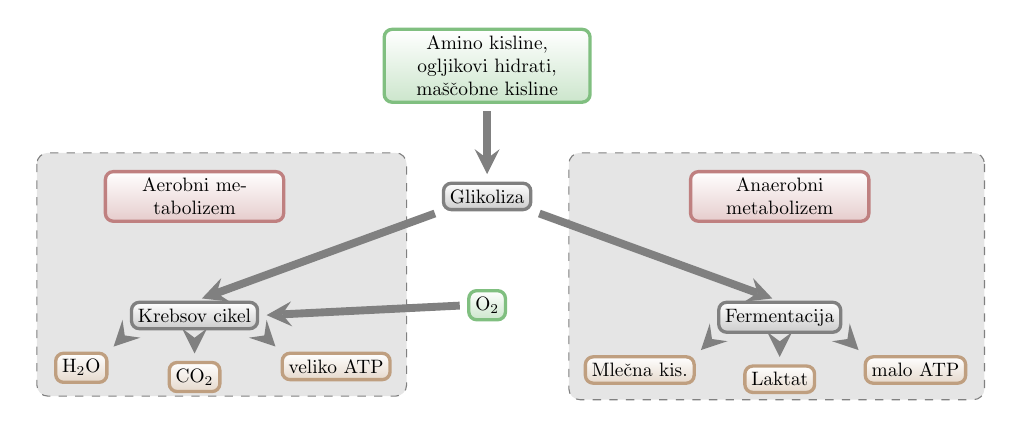
\begin{tikzpicture}
  % LAYERS
  \pgfdeclarelayer{bg}
  \pgfsetlayers{bg,main}
  % LENGTHS
  \newlength{\outdistance}
  \setlength{\outdistance}{4mm}
  %STYLES
  
    
  %
  % Specification of nodes
  %
  \node (food) [input, text width=35mm] {Amino kisline, ogljikovi hidrati, maščobne kisline};
  \node (glycolysis) [block, below = of food] {Glikoliza};
  \node (o2) [input, below = of glycolysis] {O$_2$};
  
  \node (aerobic) [title, left = 2cm of glycolysis] {Aerobni metabolizem};
  \node (krebs) [block, below = of aerobic] {Krebsov cikel};
  \node (aerobic-atp) [output, below right = \outdistance of krebs] {veliko ATP};
  \node (h2o) [output, below left = \outdistance of krebs] {H$_2$O};
  \node (co2) [output, below = \outdistance of krebs] {CO$_2$};
  
  \node (anaerobic) [title, right = 2cm of glycolysis] {Anaerobni metabolizem}; 
  \node (ferment) [block, below = of anaerobic] {Fermentacija};
  \node (anaerobic-atp) [output, below right = \outdistance of ferment] {malo ATP};
  \node (acid) [output, below left = \outdistance of ferment] {Mlečna kis.};
  \node (lactat) [output, below = \outdistance of ferment] {Laktat};
  
  %
  % Specification of lines
  %
  \draw [arrow] (food.south) -- (glycolysis.north);
  \draw [arrow] (glycolysis.south west) -- (krebs.north);
  \draw [arrow] (glycolysis.south east) -- (ferment.north);
  \draw [arrow] (o2.west) -- (krebs.east);
  
  \draw [arrow] (krebs.south west) -- (h2o.north east);
  \draw [arrow] (krebs.south) -- (co2.north);
  \draw [arrow] (krebs.south east) -- (aerobic-atp.north west);
  
  \draw [arrow] (ferment.south west) -- (acid.north east);
  \draw [arrow] (ferment.south) -- (lactat.north);
  \draw [arrow] (ferment.south east) -- (anaerobic-atp.north west);
  
   %
  % Background
  %
  \begin{pgfonlayer}{bg}
  	\node (ltop) [above = 1mm of aerobic] {};
    \node (lleft) [left = 1mm of h2o] {};
  	\node (l0) [] at ( ltop -| lleft) {};
    \node (l1) [below right = 1mm of aerobic-atp] {};
    \path[background] (l0) rectangle (l1);
    
    \node (rtop) [above = 1mm of anaerobic] {};
    \node (rright) [right = 1mm of anaerobic-atp] {};
    \node (r0) [] at (rtop -| rright) {};
    \node (r1) [below left = 1mm of acid] {};
    \path [background] (r0) rectangle (r1);
  \end{pgfonlayer}
\end{tikzpicture}
}
 \caption[Diagram aerobnega in anaerobnega metabolizma]{Diagram aerobnega in anaerobnega metabolizma. Pri aerobnem metabolizmu formacija ATP poteka preko glikolize in Krebsovega cikla, kjer se porablja kisik~\cite{scott2005misconceptions}. Pri anaerobnem metabolizmu se ATP formirajo preko glikolize in fermentacije.}
 \label{fig:metabolism}
\end{figure}

\section{Merjenje energijske porabe}\label{sec:merjenje}
Zaradi kompleksne narave fizične aktivnosti je merjenje energijske porabe velik metodološki izziv~\cite{zhang2004improving}. Zhang et al.~\cite{zhang2004improving} pri tem izpostavlja, da je pomemben del tega problema različen življenjski slog posameznika. 

%Kot smo razložili v poglavju~\ref{sec:energija} je energijska poraba pravzaprav toplota, ki izhaja iz energijskih procesov mišičnih celic~\cite{scott2005misconceptions}. 
Energijsko porabo lahko določimo z merjenjem toplotnih izgub med subjektom in kalorimetrom, saj se teoretično vsa mehanična energija v izoliranem sistemu pretvori v toploto~\cite{levine2005measurement}. Tovrstno merjenje imenujemo \emph{direktna kalorimetrija}~\cite{levine2005measurement}. Merilne naprave za direktno kalorimetrijo so izjemno drage, ki jih uporabljajo le visoko specializirani laboratoriji~\cite{levine2005measurement}. Obstaja več tipov naprav, za vse pa je značilno, da gre za komore, ki zagotavljajo toplotno ravnovesje. Odzivni časi so dokaj dolgi in lahko trajajo do \SI{30}{\min}, merilna napaka pa se giblje med \hbox{\SIrange{1}{2}{\%}}~\cite{levine2005measurement}.

Toplota v človeškem telesu nastaja zaradi aerobnega ali anaerobnega metabolizma~\cite{scott2005misconceptions}. Ker ima anaerobni metabolizem nizko kapaciteto in traja kratek čas~\cite{sahlin1998energy}, se je v športu bolj uveljavilo merjenje aerobne kapacitete~\cite{scott2005misconceptions,howley1995criteria}. Pri aerobnem metabolizmu se za produkcijo toplote porablja kisik, zato lahko energijsko porabo posredno merimo s porabo kisika (${VO}_2$)~\cite{scott2005misconceptions}. Tako merjenje imenujemo \emph{indirektna kalorimetrija}~\cite{levine2005measurement}. Merilne naprave so glede na direktno kalorimetrijo cenejše in manj kompleksne. Večinoma gre za naprave z masko, ki mora biti fiksirana na nos in usta~\cite{levine2005measurement}, zato niso primerne za široko uporabo ali izven-laboratorijske raziskave. Z merilnimi napakami pod \SI{3}{\%} in dokaj hitrimi odzivnimi časi prekašajo metode direktne kalorimetrije~\cite{levine2005measurement}.

Za potrebe terenskih raziskav se je razvila tretja skupina merilnih tehnik, t.i. \emph{nekalorimetrične metode}~\cite{levine2005measurement}. Energijska poraba nastaja zaradi gibanja telesa, zato se nekalorimetrične metode osredotočajo na opazovanje kinematike in ostalih fizioloških parametrov, ki sodelujejo pri fizičnih aktivnostih~\cite{levine2005measurement}. Sem sodijo meritve srčnega utripa, elektromiografija, uporaba pedometrov in pospeškometrov ter brezkontaktne metode.

\subsection{Srčni utrip}\label{sec:srcni-utrip}
Pri zmerni fizični aktivnosti obstaja linearna povezava med srčnim utripom in porabo kisika~\cite{keytel2005prediction}. Kar pa težko rečemo za odnos do energijske porabe, saj obstaja velika varianca med posamezniki~\cite{levine2005measurement}. Ta je odvisna od fizioloških parametrov, kot so spol, višina, teža in telesna pripravljenost. Prav tako na pravilno estimacijo energijske porabe iz srčnega utripa vplivajo emocije in okoljske spremembe~\cite{keytel2005prediction}. Srčni utrip lahko zato uporabimo le v ozkem področju med \SI{90}{bpm} in \SI{150}{bpm}. Vendar tudi tu lahko dobimo razlike na intervalu $[-20~\% , 25~\%]$ glede na meritve indirektnih metod~\cite{keytel2005prediction}. 

Ker je srčni utrip zelo slab posrednik za estimacijo energijske porabe, so raziskovalci predlagali modele, ki upoštevajo dodatne fiziološke parametre~\cite{charlot2014improvement}. Najbolj pogosto citirana modela, ki se uporabljata tudi za široko populacijo, sta \emph{Keytelova modela}~\cite{keytel2005prediction}. Pri prvem modelu~\eqref{eq:keytel1} moramo za izračun energijske porabe $W_p$ [\si{\kcal\per\min}] poznati spol $s$ ($1$ moški, $0$ ženska), starost $st$ [leto], težo $m$ [\si{\kg}], srčni utrip $hr$ [\si{bpm}] in maksimalno porabo kiska merjenca \vomax [\si{\ml\per\kg\per\min}]. Korelacijski koeficient $CORR$ tega modela glede na indirektno kalorimetrijo znaša \num{0.812}~\cite{charlot2014improvement}.

\begin{align} \label{eq:keytel1}
W_p = & \num{-59.3954} + s~(\num{-36.3781} + \num{0.271}~st + \num{0.394}~m  \nonumber \\
& + \num{0.404}~v + \num{0.634}~hr ) + (1 - s) \nonumber \\
&\cdot (\num{0.274}~st + \num{0.103}~m + \num{0.380}~VO_{2max} + \num{0.450}~hr)
\end{align}

Drugi Keytelov model~\eqref{eq:keytel2} ne upošteva maksimalne porabe kisika \vomax, ki nam pogosto manjka, in je zato manj točen~\cite{keytel2005prediction}. Njegov korelacijski koeficient \corr znaša \num{0.632}~\cite{charlot2014improvement}.

\begin{align}\label{eq:keytel2}
 W_p = & s~(\num{-55.0969} + \num{0.6309}~hr + \num{0.1988}~m + \num{0.2017}~st) \nonumber \\
 & + (1 - s) \cdot (\num{-20.4022} + \num{0.4472}~hr - \num{0.1263}~m + \num{0.074}~st)
\end{align}

Charlot et al.~\cite{charlot2014improvement} je z uporabo drugačnih parametrov izboljšala rezultate glede na drugi Keytelov model. Model~\eqref{eq:charlot} je tako dosegel korelacijski koeficient $\corr= \num{0.657}$. Pri tem modelu moramo za izračun energijske porabe $W_p$ [\si{\kcal\per\hour}]  poznati srčni utrip $hr$ [\si{bpm}], višino $h$ [\si{\cm}], težo $m$ [\si{\kg}], spol $s$ ($1$ moški, $2$ ženski), srčni utrip v mirovanju $hr_r$ [\si{bpm}] in teoretični maksimalni srčni utrip \hrtmax [\si{bpm}]~\cite{charlot2014improvement}. Srčni utrip v mirovanju je definiran kot srednja vrednost srčnega utripa zadnjih dveh minut pet minutnega mirovanja v ležečem položaju. Teoretični maksimalni srčni utrip lahko izračunamo na več različnih načinov. Najbolj pogosto uporabljena enačba za izračun je~\eqref{eq:hrtmax1}, vendar pa obstajajo bolj natačni modeli, kot je enačba~\eqref{eq:hrtmax2}~\cite{miller1993predicting}. 

\begin{align}\label{eq:charlot}
W_p = & \num{171.62} + \num{6.87}~hr + \num{3.99}~h + \num{2.3}~m \nonumber \\
& - \num{139.89}~s - \num{4.26}~hr_r - \num{4.87}~hr_{tmax}
\end{align}

\begin{align}
	hr_{tmax} = & \num{220} - st \label{eq:hrtmax1}\\ 
    hr_{tmax} = & 217 - \num{0.85}~st \label{eq:hrtmax2}
\end{align}

Slaba lastnost modela~\eqref{eq:charlot} je, da energijsko porabo računamo na urni interval in ne na minutnega, kot je običajno. Pri pretvorbi v minutni interval dobimo približek, saj s tem upoštevamo konstantno vrednost energijske porabe na intervalu $1$ ure. 





\subsection{Senzorji gibanja}\label{sec:senzorji-gibanja}

Za predikcijo energijske porabe iz opazovanja kinematike se večinoma uporabljajo pedometri in pospeškometri~\cite{levine2005measurement}. Pedometri zaznajo premike z vsakim korakom, vendar pa imajo probleme z občutljivostjo. Ker z njimi ne moremo določiti dolžine koraka, so zelo slabi prediktorji in se za tovrstna merjenja ne uporabljajo~\cite{levine2005measurement}.

Merjenje s pospeškometri je lahko dokaj natančno, saj je pospešek sorazmeren zunanjim silam in zato odraža intenziteto gibanja~\cite{yang2010review}. Pri tem moramo paziti, da uporabimo triosne in ne enoosnih pospeškometrov, saj ti ne dajejo zadovoljivih rezultatov~\cite{levine2005measurement}. Pospeškometri se lahko uporabljajo tako za laboratorijske kot tudi za terenske raziskave~\cite{yang2014sleep}, vendar pa, kot pravi Zhang et al~\cite{zhang2004improving}, je njihova natančnost vprašljiva. Faktorji, ki vplivajo na njihovo natančnost, so lokacija, način pritrditve na telo in zunanje vibracije~\cite{yang2010review}. Priporočljivo je, da jih pritrdimo na spodnji del hrbta, saj bomo le tako zajeli večino premikov težišča telesa pri aktivnostih. Za bolj natančne meritve bi morali pospeškometre pritrditi tudi na druge dele telesa, še posebej na okončine~\cite{yang2010review}. To zmanjšuje njihovo praktičnost, saj omejujejo gibanje športnikov in s tem posredno vplivajo na rezultat. Pospeškometri imajo še eno slabo lastnost. Njihova natančnost močno upade, kadar gibanje ni horizontalno s podlago, kar pomeni, da so neuporabni za hojo ali tek v hrib, plezanje, itd.~\cite{yang2010review}.

Za primer študije, ki uporablja kontaktne metode, lahko navedemo~\cite{gjoreski2015context}. V tem delu so avtorji določali energijsko porabo z regresijskimi modeli. Te so učili na večdimenzionalnih vektorjih značilk iz kontaktnih senzorjev.





\subsection{Brezkontaktne metode}

Zaradi omejitev kontaktnih senzorjev, slabih lastnosti srčnega utripa in drage indirektne kalorimetrije, ki se lahko uporablja samo v laboratoriju, so raziskovalci razvili brezkontaktne metode estimacije energijske porabe, kjer dominirajo metode analize video posnetkov~\cite{botton2011energy,osgnach2010energy,silva2015assessing,peker2004framework,nathan2015estimating}. 

\section{Prispevek dela}
Nobena od brezkontaktnih metod estimacije energijske porabe ne izkorišča polja gibanja. To je najbolj optimalna rešitev za sisteme računalniškega vida, ki merijo energijsko porabo, saj je povezana s kinematičnim gibanjem. Polja gibanja ne moremo direktno meriti, zato uporabljamo njegovo aproksimacijo, optični tok. Uporaba optičnega toka, je zagotovo lahko bolj natančna od do sedaj predlaganih metod. Seveda tak pristop na podlagi natančnosti ne more nadomestiti indirektne kalorimetrije, lahko pa nadomesti široko uporabljene kontaktne senzorje. Metoda je v primerjavi s kontaknimi senzorji tudi bolj praktična, saj ti omejujejo gibanje in s tem posredno vplivajo na rezultat. 

Pri uporabi optičnega toka lahko veliko elementarnih problemov, kot so problem reže in paralaksa gibanja, rešimo z vpeljavo skrbno izbranih deskriptorjev. Tako lahko metodo uporabimo pri različnih modalitetah. Energijsko porabo lahko merimo z različnih zornih kotov, pa tudi z različnimi tipi kamer kot so: RGB, infrardeče (IR) in globinske kamere (RGB-D). Z uporabo deskriptorjev lahko v postopek pridobivanja energijske porabe učinkovito integriramo regresijske modele s strojnim učenjem na podlagi podpornih vektrojev in parametrično optimizacijo mrežnega iskanja. 

Vsekakor optični tok ni edini aproksimator polja gibanja. Koncept lahko razširimo na tri dimenzionalni prostor z uporabo prostorskega toka. S slednjim lahko močno izboljšamo natančnost postopka, saj dobimo podatke v metričnih enotah. Tudi deskriptorje, ki jih uporabljamo za večjo robustnost optičnega toka, lahko razširimo na več dimenzij in tako obdržimo temeljni del postopka.

Kljub specifični uporabi predlagane metode za merjenje energijske porabe, bi lahko tako metodo uporabili tudi za druge principe gibanja. Koncept merjenja s pomočjo optičnega toka nam omogoča, da opravljamo meritve z daljših razdalj, dokler nam optični sistem zagotavlja stabilno sliko. Tako smo se za prikaz posplošitve našega sistema odločili, da bomo preizkusili naš sistem kot detektor dihanja, saj dihanje, kot gibanje, ravno tako predstavlja vrsto telesne aktivnosti. Detekcija dihanja je podrobneje predstavljena v poglavju~\ref{sec:detekcija-dihanja}

Predlagana metoda za estimacijo intenzitete fizične aktivnosti bazira na karakteristikah video posnetkov. Lahko jo uporabljamo kot popolnoma nemoteč, brezkontakten merilni instrument. V poglavju~\ref{sec:metode}  predstavljamo metode, ki smo jih uporabili v postopku predikcije dihanja in predikcije energijske porabe. V poglavju~\ref{sec:eksperimenti} so opisani eksperimenti in njihovi rezultati. Na koncu sledi še diskusija, kjer ovrednotimo rezultate. 
\section{Podobna dela}\label{sec:podobna-dela}



\subsection{Subjektivna primerjava aktivnosti gibanja}\label{sec:subjektivna-primerjava}

Peker et al.~\cite{peker2004framework} zagovarja stališče, da je intenziteta aktivnosti pri opazovanju video posnetkov subjektivna meritev. Pri opazovanju gibanja v video posnetkih bo vsaka oseba zaznala drugačno intenziteto. Vsekakor pa bodo vsi prepoznali hojo kot nizko intenziteto, tek pa visoko intenziteto aktivnosti. Na podlagi tega so zato v delu~\cite{peker2004framework} predstavili izvedbo psihofizičnega protokola za primerjavo meritev intenzitete aktivnosti s pomočjo subjektivne reference.

Subjektivni zlati standard so v~\cite{peker2004framework} določili s 15 merjenci, ki so določevali intenziteto gibanja $294$ video posnetkov dolžine \SI{1.5}{\s} z lestvico od najmanjše do največje intenzitete $0$--$5$. Na podlagi strinjanja o intenziteti gibanja med subjekti so izračunali mediano in jo uporabili za zlati standard. Glede na standard so avtorji~\cite{peker2004framework} primerjali $9$ različnih deskriptorjev, izpeljanih iz vektorjev gibanja. Ugotovili so, da je pravilnost estimacije odvisna od razdalje gibajočih oseb od kamere~\cite{peker2004framework}. Prav tako na pravilnost vpliva tresenje kamere. Na podlagi primerjave srednje napake med deskriptorji so ugotovili, da so MPEG-7 deskriptorji gibanja primerni za uporabo v tovrstni problematiki~\cite{peker2004framework}.

Fiziologija gibanja je v~\cite{peker2004framework} popolnoma izključena. Tu gre zgolj za primerjave med deskriptorji in grobo subjektivno oceno intenzitete aktivnosti, ki ne daje nobenih oprijemljivih informacij. Predstavlja dobro usmeritev za uporabo deskriptorjev za namene ocene intenzitete aktivnosti. Ti naj bi temeljili na polju gibanja, ki je tudi najtesneje povezan s fiziologijo. Prav tako opisuje zametke problematike merjenja intenzitete aktivnosti, ko opisuje odvisnost estimacije od razdalje oseb od kamere in njeno premikanje.




\subsection{Predikcija tipov fizične aktivnosti z video analizo}

V študiji~\cite{silva2015assessing} so evaluirali avtomatski sistem za video analizo. S predikcijo tipov fizične aktivnosti so želeli pokazati, da so določene metode računalniškega vida, kot je segmentacija slik, detekcija in sledenje igralcev z uporabo Kalmanovega filtra, ravno tako primerne za določevanje fizične aktivnosti kot pospeškometri in orodja za ročno označevanje.

Za eksperimente je Silva et al.~\cite{silva2015assessing} uporabil 8 košarkarjev, ki so igrali \SI{20}{minutno} igro. Košarkarji so imeli okoli pasu pritrjen pospeškometer Actigraph GT3X+, ki je služil za zlati standard. Za ročno označevanje so uporabili orodje SOPLAY, pri čemer so uporabili dva operaterja (SOPLAY 1 in SOPLAY 2)~\cite{silva2015assessing}. Video sistem (CAM) je bil sestavljen iz ene kamere Gigabit Ethernet camera DFK 31BG03.H, ki je bila pritrjena na strop igrišča. Uporabili so širokokotno lečo Computar T2Z1816CS z goriščnimi razdaljami \SIrange{1.8}{3.6}{\mm}~\cite{silva2015assessing}. Snemali so z resolucijo $1024 \times 768$ in \SI{30}{fps}. S sledenjem igralcev v koordinatnem sistemu igrišča so določili njihove hitrosti~\cite{silva2015assessing}. Na podlagi tega so določili tri tipe fizične aktivnosti in sicer:

\begin{itemize}
\item lahka fizična aktivnost ($<$\SI{0.9}{m.s^{-1}}),
\item hoja (\SI{0.9}{m.s^{-1}}--\SI{1.8}{m.s^{-1}}) in
\item fizična aktivnost velike intenzitete ($>$\SI{1.8}{m.s^{-1}})
\end{itemize}

Rezultati dela~\cite{silva2015assessing} so prikazani v tabeli~\ref{tab:silva}. Raziskovalci so ugotovili, da avtomatski sistem za video analizo deluje bolje od ročnega označevanja.

\begin{table}[!htb]
	\centering
    \begin{tabular}{l S[table-format=2.2] S[table-format=1.2]}
    \toprule
    \textbf{Metoda} & \theadm{\chi^2} & \theadm{e~[\si{\%}]} \\
    \midrule
    SOPLAY 1 & 77.60 & 8.68  \\
    SOPLAY 2 & 93.10 & 9.60 \\
    \textbf{CAM} & \boldentry{2}{2}{36.40} & \boldentry{1}{2}{5.32} \\
    \bottomrule
    \end{tabular}
    \caption[Rezultati Silva et al. metod]{Rezultati ročnega anotiranja prvega operaterja (SOPLAY 1), ročnega anotiranja drugega operaterja (SOPLAY 2) in avtomatskega sistema za video analizo (CAM) iz~\cite{silva2015assessing}. Za metriko so uporabili $\chi^2$ in srednjo procentualno napako (e). V tabeli so prikazani samo rezultati primerjave s podatki pospeškometra GT3X. Najboljša metoda je odebeljena.}
    \label{tab:silva}
\end{table}

Za razliko od dela v poglavju~\ref{sec:subjektivna-primerjava} v~\cite{silva2015assessing} že uporabijo objektivne metode, ki ne temeljijo na posameznikovi percepciji intenzivnosti fizične aktivnosti. Avtorji so v delu kategorizirali intenzitete aktivnosti v tri tipe glede na hitrost. V tem pogledu gre le za grobo oceno intenzitete. Temelji na premikanju masnega centra, saj ne opazujejo celotnega telesa. Za bolj jasno evaluacijo v~\cite{silva2015assessing} manjkajo uveljavljeni zlati standardi z indirektno metodo. Tu so zlati standard določili s pospeškometri, ki imajo že sami po sebi probleme pri estimaciji, kot smo opisali v~\ref{sec:senzorji-gibanja}.




\subsection{Ocena energijske zahtevnosti igranja nogometa}

V delu~\cite{osgnach2010energy} so avtorji pokazali, da lahko z video analizo in fizikalnim modelom ocenimo energijsko zahtevnost igranja nogometa. Nogomet vsebuje tako aerobne kot anaerobne elemente energijske porabe. Kot navaja Osgnach et al.~\cite{osgnach2010energy}, je obremenitev igralcev na tekmo okoli \SI{70}{\%} maksimalne aerobne kapacitete (\vomax). Ti na tekmo porabijo \SIrange{1200}{1500}{\kcal}. 

Čeprav so metode, s katerimi so ocenili energijsko porabo in obremenitev v nogometu, zanesljive, ni bilo razvite še nobene, ki bi merila trenutno porabo~\cite{osgnach2010energy}. Takšna metoda bi bila bistveno bolj natančna, saj je energijski profil tega športa bistveno bolj razvejan, kot standardne meritve konstantnega teka na tekalni stezi. Igralci so tako \SI{70}{\%} tekme v nizki intenziteti porabe energije (hitra hoja in lahkoten tek), ostalo pa v visoki intenziteti, kamor spada sprint~\cite{osgnach2010energy}. 

Osgnach et. al~\cite{osgnach2010energy} zagovarja stališče, da največji del metabolične obremenitve nastane pri pospeševanju in zaviranju, zato so razvili fizikalni model, s katerim lahko določijo energijsko porabo glede na hitrost in pospeške~\cite{osgnach2010energy}. Model predvideva, da sta konstanten tek v hrib in sprint ekvivalentna, saj se telo v času sprinta nagne za določen kot glede na tla.  

Za izračun energijske porabe igralca v \SI{90}{\min} tekmi, so snemali $56$ tekem, kjer je sodelovalo $399$ igralcev~\cite{osgnach2010energy}. Pozicije igralcev v času tekme so določili s polavtomatskim sistemom SICS, ki uporablja štiri \SI{25}{\Hz} kamere. Merilna napaka je bila \SI{1.0}{\%}. Zmogljivost posameznega igralca so določili s tremi parametri, ki so jih razdelili na posamezne kategorije~\cite{osgnach2010energy}:

\begin{itemize}
\item hitrost ($6$ kategorij),
\item pospešek ($8$ kategorij) in
\item metabolična moč ($5$ kategorij).
\end{itemize}

Avtorji so v~\cite{osgnach2010energy} določili, da igralec na tekmo porabi $1107 \pm 119$~kcal, kar ustreza opažanju ostalih raziskovalcev. Ugotovili so, da je energijska poraba pri različnih hitrostih podobna, saj naj bi bila bolj odvisna od pospeševanja in zaviranja. Ker so tu računali energijsko porabo le iz teka, niso upoštevali drugih aktivnosti, kot je skakanje, brcanje žoge, itd. Delo ne zajema nobene primerjave modela z referenčnimi podatki energijske porabe, zato ne moremo z gotovostjo trditi o njegovi pravilnosti. Metoda uporabe fizikalnega modela je omejena na tek, zato ga ne moremo uporabiti za vrsto drugih aktivnosti.





\subsection{Merjenje aktivnosti v tenisu}

Tako kot nogomet je tudi tenis kompleksen šport, kjer se uporabljata anaerobni in aerobni metabolizem~\cite{botton2011energy}. Obremenitve so tu nekoliko manjše, saj dosegajo ravni $<$ \SIrange{60}{70}{\%} \vomax. Tudi pri tenisu so estimacije srednje vrednosti energijske porabe neprimerne, saj profil intenzitete fizične aktivnosti ni konstanten. V delu~\cite{botton2011energy} so zato razvili metodo estimacije energijske porabe s pomočjo metaboličnih modelov elementarnih aktivnostih. 

Maksimalno aerobno kapaciteto igralcev (\vomax) so določili z inkrementalnim testom na sobnem kolesu Monark 824 z 80 rpm in \SI{20}{W.\min^{-1}} povečevanjem, s čimer so dosegli izčrpanost pod \SI{17}{\min}~\cite{botton2011energy}. Za referenčno določanje porabe kisika (\vo) med testi so uporabili prenosni sistem za analizo plinov K4B2. 

Profil tenisa so v~\cite{botton2011energy} razdelili na $5$ elementarnih aktivnosti: hoja, tek, sedenje, udarci z loparjem in serviranje. S pomočjo merjenja porabe kisika, z linearnim naraščanjem hitrosti hoje in teka ter linearnim naraščanjem frekvence udarcev so določili linearne metabolične modele za posamezno elementarno aktivnost. Z njimi so računali metabolično moč. Pri tem so uporabili $8$ teniških igralcev~\cite{botton2011energy}. Metabolične modele so uporabili v poenostavljenih matematičnih ASTRABIO modelih za opisovanje porabe kisika, aerobne in anaerobne porabe energije, glede na čas izvajanja elementarne aktivnosti. 

Čas izvajanja posameznih aktivnosti so določili s snemanjem in video analizo tekme s Canon MVI 850i digitalno kamero s Canon A28 širokokotno lečo~\cite{botton2011energy}. Kamera je bila postavljena %\SI{6}{m} za igriščem in \SI{5.55}{m} visoko 
tako, da je pokrivala igrišče do mreže. 

Z merjenjem $16$ iger so dobili za estimacijo porabe aerobne energije korelacijski koeficient $\corr =\num{0.93}$~\cite{botton2011energy}. Srednja vrednost porabe kisika je za model znašala \SI{51.7 \pm 10.5}{\%} \vomax. Izmerjena srednja vrednost je bila \SI{52.0 \pm 9.1}{\%} \vomax. Poleg tega so lahko 
v~\cite{botton2011energy} posebej določili aerobno in anaerobno porabo energije. Ugotovili so, da je bilo anaerobne porabe \SI{30}{\%} celotne energije, v času serviranja in udarcev z loparjem pa se je povečala na \SI{95}{\%}.  

Sama metodologija v~\cite{botton2011energy} dokaj natančno določi energijsko porabo za posamezne tipe aktivnosti. Prav tako z različnimi modeli omogoča predikcijo porabe kisika ter anaerobne in aerobne porabe energije. Validacija modelov je trdna, saj so jih avtorji primerjali s standardno indirektno kalorimetrijo. Kljub temu lahko v uporabi metaboličnih modelov opazimo nekaj pomanjkljivosti. Razvoj metaboličnih modelov ni trivialen in zahteva precej časa. Prav tako je omejen na specifično vrsto športa, ki vsebuje elementarne aktivnosti. Te so s stališča računalniškega vida težje določljive in otežujejo razvoj avtomatskih metod, kjer ne potrebujemo operaterjev.




\subsection{Ocena energijske porabe s Kinect senzorji}

Nathan et al.~\cite{nathan2015estimating} je poskušal oceniti energijsko porabo z Microsoft Xbox Kinect V1. Gre za sistem zajemanja gibanja brez markerjev, kjer se uporablja globinska kamera s strukturirano svetlobo~\cite{nathan2015estimating}. Pridobivanje podatkov s tako napravo je nevsiljivo, zato se merjenec lahko premika svobodno in naravno. 

V~\cite{nathan2015estimating} so napravo uporabili za snemanje skeletnega modela in modeliranja energijske porabe iz mehaničnega dela. Za eksperimente so uporabili $2$ Kinect kameri v razmiku \SI{60}{\stopinj} glede na merjenca. $19$ subjektov je opravljalo $4$ različne vaje najmanj $4$ minute~\cite{nathan2015estimating}. Med vajami so merjenci stoje mirovali, dokler se poraba kisika ni umirila na že prej kalibrirano stojno mirovno metabolično stopnjo. Za zlati standard so uporabili Cortex Metamax 3B avtomatski sistem za analizo plina~\cite{nathan2015estimating}.

Iz premikov posameznih segmentov skeletnega modela so v~\cite{nathan2015estimating} določili različne značilke. Med njimi so določili koncentrične in ekscentrične kontrakcije mišic za masni center, spodnje in zgornje okončine ter faktor drže. Ta je predstavljal količino dela, ki ga porabi telo za ohranitev poze~\cite{nathan2015estimating}. Za predikcijo so uporabili Gaussovo regresijo (GPR), lokalno uteženo regresijo K-najbližji sosed (KNNR) in linearno regresijo (LINR). Rezultati modelov v obliki metrik so prikazani v tabeli~\ref{tab:nathan}.

\begin{table}[!htb]
	\centering
    \begin{tabular}{l 
    S[table-format=2.3]
    S[table-format=2.2] 
    S[table-format=1.3]}
    \toprule
    \textbf{Model} & \thead{\rmse [\si{\kJ}]} & \theadm{e~[\si{\%}]} & \thead{CCC} \\
    \midrule
    \textbf{GPR} & \boldentry{2}{3}{8.384} &  35.64 & \boldentry{1}{3}{0.879} \\
    KNNR & 8.415 & 29.76 & 0.847 \\
    LINR & 10.229 & \boldentry{2}{2}{29.39} & 0.847 \\
    \bottomrule
    \end{tabular}
    \caption[Rezultati Nathan et al. modelov]{Rezultati modela Gaussove regresije (GPR), modela lokalno utežene regresije K-najbližji sosed (KNNR) in modela linearne regresije (LINR) iz dela~\cite{nathan2015estimating}. Avtorji so za prikaz rezultatov uporabili koren srednje kvadratne napake (RMSE), srednjo procentualno napako (e) in konkordančni korelacijski koeficient (CCC). Najboljši rezultati posamezne metrike in modela so odebeljeni. Najbolje se je izkazal GPR model~\cite{nathan2015estimating}.}
    \label{tab:nathan}
\end{table}

Avtorji~\cite{nathan2015estimating} so ugotovili, da z njihovo metodo lahko dobro ocenijo energijsko porabo le za aktivnosti visoke intenzitete, kot je skakanje. To omejuje uporabnost take metode, saj  so aktivnosti visoke intenzitete tudi pomembne in lahko bistveno vplivajo na rezultate~\cite{osgnach2010energy}. Prav tako je metoda omejena z opremo, saj moramo imeti senzorje, ki omogočajo razpoznavanje skeleta. Za razliko od prejšnjih del, ki temeljijo na fizičnih in metaboličnih modelih~\cite{osgnach2010energy,botton2011energy}, to metodo lahko apliciramo na različne športe. 


\input{\folder/05-detekcija-dihanja.tex}

%*********************** OSREDNJA POGLAVJA ********************************
\input{./pogl/02-metode/00-metode.tex}
\chapter{Implementacija metod}
V tem poglavju so opisane implementacije nekaterih metod, opisanih v poglavju~\ref{sec:metode}. Gre za tiste metode, kjer iz teoretične podlage implementacija ni bila točno razvidna. Opisane so tudi metode, ki nimajo teoretične podlage, saj gre samo za specifično implementacijo.

\subsection{Optični in prostorski tok}
Na podlagi opisanih lastnosti metod optičnega toka v poglavju~\ref{sec:metode-of} smo se odločili, da bomo v tem delu uporabili diferencialno metodo. Kljub višji računski zahtevnosti, ki ob današnji tehnologiji ne predstavlja več takega problema, smo želeli računati gost optični tok. Z gostim optičnim tokom dobimo natančno aproksimacijo polja gibanja za celotno telo. Prav tako nimamo problemov pri estimaciji energijske porabe za hitre gibe, kot bi bilo to v primeru uporabe ujemalnih metod. Ker je glavni namen uporaba in ne implementacija diferencialne metode, smo se osredotočili na Farneb{\"a}ck algoritem, ki je dostopen v knjižnici OpenCV 3.1.0.

Za optični tok smo uporabili sledeče parametre: piramidna skala $pyr\_scale=\num{0.5}$, število piramidnih slojev $levels=3$, velikost okna povprečenja $winsize=15$, število iteracij na vsakem piramidnem sloju $iterations=3$, velikost okolice slikovnih elementov $poly\_n=5$ in Gaussov standardni odklon $poly\_sigma=\num{1.2}$.

Z uporabo prostorskega toka lahko bolje opišemo mehanično delo kot pri uporabi optičnega toka. Vsekakor pa potrebujemo dodatno informacijo, ki jo moramo pridobiti iz slikovnih podatkov. Za ta namen smo uporabili t.i. ``Time-of-Flight'' (ToF) kamere, ki so vgrajene v poceni Microsoft Kinect for Windows V2 senzor~\cite{Yang2015KinectV2}. Z njim pridobivamo registrirane RGB-D (rdeče, zelene, modre in globinske) podatke. Za pridobitev prostorskega toka smo uporabili PD-Flow algoritem. Njegova implementacija je javno dostopna~\cite{jaimez2015primal}. Podrobneje je opisan v poglavju~\ref{sec:pd-flow}.



\subsection{Sledilniki}
Pri izbiri sledilnikov smo se osredotočili na pogoje, ki jim morajo sledilniki v največji meri zadostiti. Sledilnik mora dobro slediti osebam, ostali objekti niso pomembni. Sledenje mora biti zanesljivo, saj je od njega odvisna merilna napaka. Pri tem moramo upoštevati delovanje tudi v primerih, kadar tarča izgine iz slike. Sledenje mora delovati čim daljši čas tako, da ne potrebujemo ponovne inicializacije. Inicializacijo sledilnika moramo opraviti samo na prvi sliki zaporedja, kar pomeni, da mora sledilnik vsebovati indirektno učenje (angl. offline training). Zaradi uporabe sledilnika v merilnem instrumentu mora ta delovati čim hitreje. Ker namen tega dela ni implementacija sledilnika, mora biti ta implementiran v prosto dostopni izvorni kodi. 

Pri uporabi optičnega toka smo najprej preizkusili sledilnik TLD avtorja Kalal et al.~\cite{kalal2012tracking}. Prosto dostopne so tri implementacije sledilnika, in sicer v knjižnici ccv (CCV-TLD), v knjižnici OpenCV (OPENCV-TLD) in c++ izvorna koda (NEBEHAY-TLD). Implementaciji iz knjižnic ccv in OpenCV se nekoliko razlikujeta od izvirnega dela~\cite{kalal2012tracking}, NEBEHAY-TLD pa je samo prepis Matlabove izvorne kode.  Ker ni nobena implementacija zadovoljivo delovala na testnih squash posnetkih, smo poskusili še s sledilnikoma KCF~\cite{danelljan2014adaptive} in DLIB-CORR~\cite{danelljan2014accurate}. KCF je implementiran v knjižnici OpenCV, DLIB-CORR pa v knjižnici Dlib~\cite{king2009dlib}.

Testiranje sledilnikov je opisano v poglavju~\ref{sec:testiranje-sledilnikov-za-opticni-tok}, rezultati pa v poglavju~\ref{sec:rezultati-sledilnikov-za-opticni-tok}. Ugotovili smo, da najbolje deluje sledilnik KCF. Tega smo tudi uporabili v naših nadaljnjih eksperimentih.

Pri uporabi prostorskega toka smo preizkusili in uporbili DS-KCF sledilnik avtorja Hannuna et. al~\cite{hannuna2016ds}. Sledilnik uporablja RGB in globinske slike.


Rezultat sledenja je pri obeh uporabljenih sledilnikih (KCF in DS-KCF) okvir opazovanega subjekta. Notranjost okvirja uporabljamo za zapolnitev histogramov v deskriptorjih, preostanek toka v prizorišču zavržemo. Algoritma sledenja smo potrebovali za terenske teste, kjer položaj igralca ni znan. Kljub skrbni izbiri algoritmov je to najmanj robusten del našega pristopa---če sledilnik za posamezen časovni interval ne detektira igralca, manjkajo podatki na tem intervalu, razen če smo sledenje nadzorovali in odpravljali napake. Sledilnik ne detektira igralca kadar:

\begin{itemize}
	\item{Algoritem signalizira, da ni zaznal tarče.}
	\item{Algoritem signalizira nizko zaupanje v rezultat (predvsem zaradi okluzij).}
	\item{Površina področja tarče je 0.}
	\item{Vsi vektorji optičnega ali prostorskega toka so ničelni znotraj področja tarče.}
\end{itemize}

Naš pristop je dovolj modularen, da lahko enostavno zamenjamo algoritme za sledenje. S kakršnimi koli napredki na področju vizualnega sledenja se bo zanesljivost naše metode izboljšala.

\subsection{Kalmanov filter}\label{sec:implementacija-kalman}
Za prostor stanj smo izbrali stanje hitrosti $v$ in pospeška $a$~\eqref{eq:stanje}. 

\begin{equation}
\vec{x}(k) = \begin{bmatrix}
					v(k) & a(k)
				\end{bmatrix}^\top 
                \label{eq:stanje}
\end{equation}

Matrika prehajanja stanj je določena z enačbo~\eqref{eq:a}.

\begin{equation}
\vec{A} = \begin{bmatrix}
				1 & 1 \\
                0 & 1
			\end{bmatrix} 
            \label{eq:a}
\end{equation}

Za matriko vhodnih stanj $G$ smo izbrali~\eqref{eq:g}, s katero modeliramo neznane vhodne parametre hitrosti $v_n$ in pospeška $a_n$ v vektorju $u$~\eqref{eq:u}. 

\begin{equation}
\vec{G} = \begin{bmatrix}
				1 & 0
			\end{bmatrix}^\top 
            \label{eq:g}
\end{equation}

\begin{equation}
\vec{u}(k) = \begin{bmatrix}
					v_{n}(k) & a_n(k)
				\end{bmatrix}^\top 
                \label{eq:u}
\end{equation}


Merilna matrika je predstavljena z enačbo~\eqref{eq:h}
\begin{equation}
\vec{H} = \begin{bmatrix}
				1 & 0
			\end{bmatrix}^\top 
            \label{eq:h}
\end{equation}

Za začetno hitrost in pospešek smo izbrali vrednost $0$, ker se naši testi večinoma začnejo v mirovanju. 

Variance šuma modela gibanja, merilnega modela in kovariančne matrike stanja smo določili z uporabo mrežnega iskanja, ki je opisan v poglavju~\ref{sec:optimizacija-svm-parametrov}. Pri tem smo uporabili labele učnih vzorcev vseh testov 1. sklopa eksperimentov za referenco, njihove pošumljene ocene pa za meritev. Varianca šuma merilnega modela je tako znašala $\sigma_\vec{z}^2 = \num{0.04}$, varianca šuma modela gibanja pa $\sigma_\vec{x}^2 = \num{456.13}$. Za kovariančno matriko predikcije smo uporabili varianco $\sigma_\vec{P}^2 = \num{456.13}$. Kovariančno matriko modela gibanja smo določili po enačbi~\eqref{eq:Q}, kovariančna matrika merilnega modela je bila določena z enačbo~\eqref{eq:R} in začetna vrednost kovariančne matrike stanja z~\eqref{eq:P}.

\begin{equation}
\vec{Q} = \vec{G} \vec{G}^\top \sigma_\vec{x}^2
\label{eq:Q}
\end{equation}

\begin{equation}
\vec{R} = \sigma_\vec{z}^2
\label{eq:R}
\end{equation}

\begin{equation}
\vec{P}(0) = \begin{bmatrix}
1 & 0 \\
0 & 1
\end{bmatrix} \sigma_\vec{P}^2
\label{eq:P}
\end{equation}










\subsection{Gaussov filter}\label{sec:implementacija-gauss}

Gaussov filter smo implementirali po enačbi~\eqref{eq:gauss}. Za velikost jedra smo določili $3\sigma$, pri čemer je standardni odklon $\sigma$ parameter. Jedro smo nato še normirali na vsoto $1$. 

Za filtriranje podatkov smo uporabili modificirano Matlabovo funkcijo \texttt{nanconv}, ki je podrobneje predstavljena v~\cite{kraus2017nanconv}. Namesto funkcije \texttt{conv2} smo v modifikaciji uporabili funkcijo \texttt{conv}.






\subsection{Združevanje slik iz dveh Kinect kamer}
Zaradi ozkega vidnega polja Kinect kamer smo za pokritje celotne širine igrišča potrebovali dve kameri. Zaporedja slik smo pred nadaljnjo obdelavo morali združiti v eno zaporedje glede na opazovanega igralca. Zajem iz posameznih kamer ni bil sinhroniziran, zato smo pred združevanjem sinhronizirali posnetka tako, da smo izbrali slike iz posameznega zaporedja z najbolj podobnimi časovnimi žigi. Časovno sinhornizirana zaporedja slik smo nato poskušali združiti s tremi različnimi metodami:  združevanje z značilkami, združevanje s kontrolnimi točkami in prilagojeno združevanje. 

Časovno sinhronizirana zaporedja slik smo naprej poskušali združiti z metodo panoramskega šivanja slik z uporabo značilk, kot je opisano v delu~\cite{brown2007automatic}. Tu smo namesto SIFT značilk uporabili SURF značilke.
Združevanje s značilkami se ni obneslo, zato smo to metodo opustili. Primer neuspelega poskusa je prikazan na sliki~\ref{fig:zdruzevanje-znacilke}.

\begin{figure}[!htb]
	\centering
	\begin{subfigure}[t]{0.45\columnwidth}
		\includegraphics[width=\columnwidth]{./Slike/matched-features.png}
		\caption{Ujemajoče SURF značilke}
		\label{fig:zdruzevanje-surf}
	\end{subfigure}
	~
	\begin{subfigure}[t]{0.45\columnwidth}
		\includegraphics[width=\columnwidth]{./Slike/features-calibration-result.png}
		\caption{Rezultat združevanja z značilkami}
		\label{fig:zdruzevanje-result}
	\end{subfigure}
	\caption[Neuspelo združevanje slik s SURF značilkami]{Primer neuspelega poskusa združevanja slik iz dveh Kinect kamer s SURF značilkami.}
	\label{fig:zdruzevanje-znacilke}
\end{figure}

Zaporedja slik smo poskušali združiti tudi z ročnim določevanjem kontrolnih točk. Rezultat {združevanja s kontrolnimi točkami} je bil boljši od združevanja z značilkami, vendar še vedno slab, zato smo tudi to metodo opustili. Primer neuspelega poskusa je prikazan na sliki~\ref{fig:zdruzevanje-cp}.

\begin{figure}[!htb]
	\centering
	\begin{subfigure}[t]{0.45\columnwidth}
		\includegraphics[width=\columnwidth]{matched-points.png}
		\caption{Ujemajoče kontrolne točke}
		\label{fig:zdruzevanje-ujemajoce-cp}
	\end{subfigure}
	~
	\begin{subfigure}[t]{0.45\columnwidth}
		\includegraphics[width=\columnwidth]{points-calibration-result.png}
		\caption{Rezultat združevanja s kontrolnimi točkami}
		\label{fig:zdruzevanje-result-cp}
	\end{subfigure}
	\caption[Neuspelo združevanje slik s kontrolnimi točkami]{Primer neuspelega poskusa združevanja slik iz dveh Kinect kamer s kontolnimi točkami.}
	\label{fig:zdruzevanje-cp}
\end{figure}

Zaradi nezadovoljivih rezultatov klasičnih metod združevanja stereo slik smo razvili metodo, ki je prilagojena za Kinect kamere. Iz kamer smo z uporabo knjižnice libfreenect2 0.2~\cite{lingzhu2016libfreenect2} pridobili intrinzične parametre bli�nje-infrardečega (NIR) senzorja, in sicer: slikovni koordinati goriščne razdalje $f_u$ in $f_v$ ter slikovni koordinati optičnega središča slike (ang. principal point) $c_u$ in $c_v$. Intrinzične parametre smo uporabili za določitev intrinzične matrike $\vec{M}_{int}$ po enačbi~\eqref{eq:intrinsic}.

Ker pravih ekstrinzičnih parametrov kamer nismo poznali, smo jih le ocenili z metodo določevanja sečišča vidnih polj obeh kamer. Sečišče je prikazano kot rdeča linija na sliki~\ref{fig:zdruzevanje}. S to metodo smo določili translacijski vektor $\vec{t} = \left [ t_x~ t_y~ t_z \right]^\top$ in rotacijsko matriko $\vec{R}$ iz Eulerjevih kotov.

S sledenjem igralca z DS-KCF algoritmom smo s pomočjo projekcijske matrike~\eqref{eq:projection-matrix} določili center tarče v metričnih enotah za vsako sliko zaporedja leve in desne kamere. Če center tarče ni vseboval podatkov globine, smo za center izbrali najbližjo točko z veljavno globino.

Prva slika združenega zaporedja je bila slika kamere, kjer se igralec prvič pojavi. Nadaljnje slike smo izbirali med zaporedjema kamer, glede na pozicijo centra tarče s histerezo, ki je na sliki~\ref{fig:zdruzevanje} prikazana z modrimi linijami. Pogled spremenimo samo takrat, ko center tarče prečka linijo histereze na igrišču. Razdalja med modrima črtama je znašala \SI{400}{mm}.


\begin{figure}[!htb]
	\centering
	\includegraphics[width=\columnwidth]{zdruzevanje-example.png}
	\caption[Določevanje sečišča vidnih polj leve in desne Kinect kamere]{Določevanje sečišča vidnih polj leve in desne Kinect kamere. Na sliki sta prikazani prvi sliki zaporedja leve in desne Kinect kamere 1. seta 2. igre terenskega eksperimenta iz 2. faze. Označen je 4. igralec. Zelena barva koordinat centra tarče predstavlja izbrano kamero. Kamera z rumeno barvo ni izbrana. Sečišče je rdeča linija. Modri liniji sta pragova za preklop med kamerama. Razdalja med njima je \SI{400}{mm}.}
	\label{fig:zdruzevanje}
\end{figure}


\chapter{Eksperimenti}\label{sec:eksperimenti}
V tem poglavju predstavljamo eksperimente, ki smo jih izvedli v dveh različnih okoljih: v fiziološkem laboratoriju in na squash igrišču (terenski testi). Z njimi smo naslovili energijsko porabo $eem(t)$, kot osrednji fiziološki parameter. Srčni utrip $hr(t)$ smo obravnavali kot sekundarni parameter, z razumevanjem, da slabo odraža dejansko energijsko porabo. Z eksperimenti detekcije dihanja smo želeli preizkusiti predlagano metodo za širšo uporabo.

Pri vseh naslovljenih fizioloških parametrih smo s pomočjo strojnega učenja izvajali predikcijo časovnih signalov $eem(t)$ za energijsko porabo, $hr(t)$ za srčni utrip in $dihanje(t)$ za dihanje. Predikcijo smo izvajali iz posamezne slike zaporedja video posnetka. Pri tem smo najprej generirali sliko optičnega ali prostorskega toka in nato določili področje, kjer se nahaja merjenec. Iz izbranega področja smo izračunali vektorje značilk $\vec{x}(t)$, te pa smo uporabili za predikcijo. Rezultat je zelo enostaven, skoraj realno-časoven model, ki ga lahko razširimo s temporalnim modeliranjem, če bi se pojavila potreba. 

Prvi del postopka je učenje SVM/SVR modela, kot je prikazano na sliki~\ref{fig:shema-generalnega-postopka01}. Na ta način dobimo parametre regresijskega modela, ki jih nato uporabimo za napovedovanje porabe energije iz testnih podatkov, kot je prikazano na sliki~\ref{fig:shema-generalnega-postopka02}.

\begin{figure}[!htb]
	\centering
	\resizebox{\columnwidth}{!}{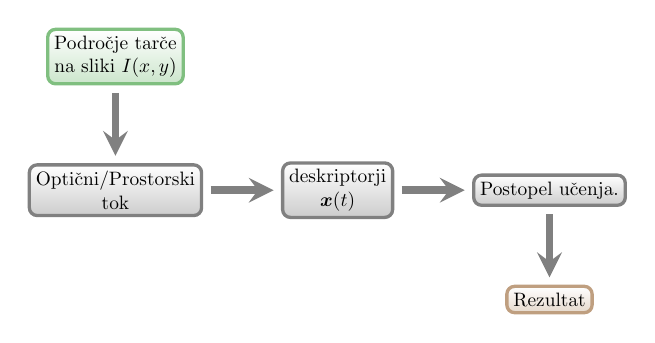
\begin{tikzpicture}
% LAYERS
\pgfdeclarelayer{bg}
\pgfsetlayers{bg,main}
\tikzset{
	between/.style args={#1 and #2}{
		at = ($(#1)!0.5!(#2)$)
	}
}

% NODES
\node (slika) [input, align=center] at (0,0) {Področje tarče\\na sliki $I(x,y)$};

\node (of) [block,align=center, below= of slika] {Optični/Prostorski\\tok};
\node (hoof) [block, align=center, right= of of] {deskriptorji\\$\vec{x}(t)$};


\node (ucenje) [block, align=center, right=of hoof] {Postopel učenja.};

\node (rezultat) [output, below= of ucenje] {Rezultat};

% arrows
\draw [arrow] (slika) -- (of);


\draw [arrow] (of) -- (hoof);
\draw [arrow] (hoof) -- (ucenje);

\draw [arrow] (ucenje) -- (rezultat);
\end{tikzpicture}}
	\caption[Shema generalnega postopka učenja]{Shema generalnega postopka učenja. Iz izbranega področja tarče generiramo sliko toka in izračunamo vekorje značilk $\vec{x}(t)$. Te nato uporabimo za učenje realno-časovnih modelov, s katerimi izvajamo predikcijo nad fiziološkimi parametri.}
	\label{fig:shema-generalnega-postopka01}
\end{figure}

\begin{figure}[!htb]
	\centering
	\resizebox{\columnwidth}{!}{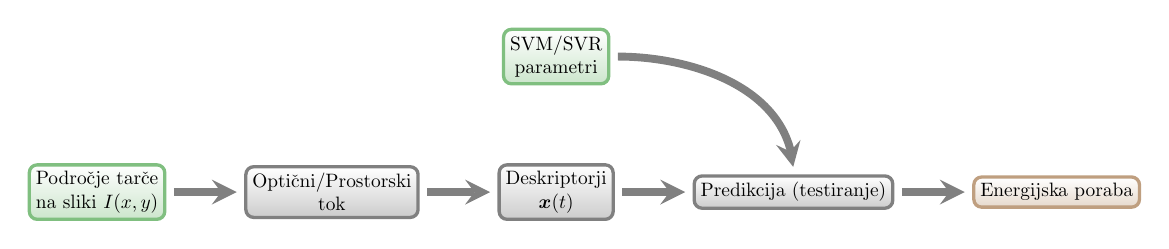
\begin{tikzpicture}
% LAYERS
\pgfdeclarelayer{bg}
\pgfsetlayers{bg,main}
\tikzset{
	between/.style args={#1 and #2}{
		at = ($(#1)!0.5!(#2)$)
	}
}

% NODES
\node (slika) [input] at (0,0) {Področje tarče\\na sliki $I(x,y)$};

\node (of) [block, right= of slika] {Optični/Prostorski\\tok};
\node (hoof) [block, right= of of] {Deskriptorji\\$\vec{x}(t)$};

\node (params) [input, above=of hoof] {SVM/SVR\\parametri};
\node (ucenje) [block, right=of hoof] {Predikcija (testiranje)};

\node (rezultat) [output, right= of ucenje] {Energijska poraba};

% arrows
\draw [arrow] (slika) -- (of);


\draw [arrow] (of) -- (hoof);
\draw [arrow] (hoof) -- (ucenje);
\draw [arrow,] (params) to[out=0,in=90] (ucenje);

\draw [arrow] (ucenje) -- (rezultat);
\end{tikzpicture}}
	\caption[Shema generalnega postopka predikcije]{Shema generalnega postopka predikcije. Vhodni podatki so testni podatki.}
	\label{fig:shema-generalnega-postopka02}
\end{figure}

Eksperimente smo kronološko razdelili na dve fazi. V \emph{1. fazi} smo analizirali observabilnost izbranih fizioloških parametrov. Parameter je observabilen, če obstaja neničelna (pozitivna) korelacija med našo estimacijo iz značilk gibanja in merjenih vrednosti, ki smo jih dobili iz zanesljivih metod pridobivanja fizioloških parametrov. %V 1. fazi smo posebej naslovili preliminarne teste, laboratorijske eksperimente tekalne steze, terenske eksperimente squash igre ter eksperimente dihanja. V {preliminarnih testih} opisujemo teste, s katerimi smo določili optimalne vrednosti parametrov. 
V \emph{eksperimentih 2. faze} smo optimizirali segmente postopka estimacije fizioloških parametrov. %Sledi končna preiskava. Končna preiskava je sestavljena iz preliminarnih testov, laboratorijske in terenske preiskave. V preliminarnih testih smo optimizirali dele postopka, s katerim smo v 1. fazi eksperimentov dobili najboljše rezultate. V laboratorijskih in terenskih preiskavah smo uporabili tri različne protokole.

\renewcommand{\folder}{./pogl/03-eksperimenti}
\section{Eksperimenti 1. faze}

\subsection{Določevanje zakasnitve fiziološkega odziva}

We explored the problem of the lag in physiological response as well. Based on Figure \ref{fig:zakasnitev}, we found out that between the change in speed of the treadmill and change of the selected physiological parameter there is a delay. This is perfectly acceptable due to the nature of physiological processes. We found out that offset for heart rate is amounted to \SI{15}{\s} and for energy expenditure to \SI{55}{\s}. Offset was included in models with the \textit{lag} abbreviation.

\begin{figure}[htb]
\centering
\begin{subfigure}[t]{0.45\columnwidth}
\includegraphics[width=\columnwidth]{./Slike/lag-estimation-train-eem.png}
\caption{Zakasnitev za energijsko porabo.}
\label{fig:lag-estimation-train-eem}
\end{subfigure}
~
\begin{subfigure}[t]{0.45\columnwidth}
\includegraphics[width=\columnwidth]{./Slike/lag-estimation-train-hr.png}
\caption{Zakasnitev za srčni utrip.}
\label{fig:lag-estimation-train-hr}
\end{subfigure}
\caption{}
\label{fig:lag-estimation-stage1}
\end{figure}


\subsubsection{Normalizacija HAFA deskriptorjev}
% Zakaj naj bi bila ta rešitev dobra
% teorija tovrstne kalibracije
% Kako s to kalibracijo nismo popravili stvari
% In da smo ugotovili da obstaja še prostorski tok, ki bi nam rešil težave
!!!!!!!!!!!!!!!!!!!!!!!!!!!!!!!

V praksi se pokaže, da normiran HAFA histogram ne... -> To paše pod eksperimente.

!!!!!!!!!!!!!!!!!!!!!!!!!!!!!!!!!!!!!!!!!


\subsection{Treadmill experiment}
The first set of experiments was performed in physiological laboratory, with subject running on a treadmill in the presence of the operator---a doctor, who determined the intensity and duration of workload. Heart rate and energy expenditure were measured for an athlete (age: 26 years, height: \SI{177}{\cm}, weight: \SI{79.1}{\kg}, $VO_2max$: \SI{3705}{\ml\per\min}). Energy expenditure was measured using indirect calorimetry with Cosmed CPET Metabolic Cart. System allows breath-by-breath measurement \cite{beaver1973line}. We used Hans Rudolph face mask with prescribed minimal VD (dead space).

\subsubsection{Data acquisition}
We filmed the treadmill from the two different angles: the side-view and the back-view. The slope of the treadmill was from \SI{1.5}{\%} to \SI{2}{\%}. We filmed in $480 \times 640$ resolution with a \SI{30}{fps} speed. An example of a recording is shown in Figure \ref{fig:moving-components}(\subref{fig:original-frame}).

\subsubsection{Procedure}
We have made two series of tests with 20 minutes between them. Physiological parameters were sampled every \SI{5}{\s}. In the first series we made 8 tests, where every test lasted for 2 minutes. The treadmill's speed was increased by \SI{1}{\km\per\hour} every test. First test had a speed of \SI{6}{\km\per\hour} and the last a speed of \SI{13}{\km\per\hour}. In the second series we made 3 tests. Every test lasted for 5 minutes. Treadmill's speeds were \SI{7}{\km\per\hour}, \SI{10}{\km\per\hour} and \SI{13}{\km\per\hour}. The first set was used for the acquisition of samples for learning, and the other for testing.

\subsubsection{Processing}
We then calculated the optical flow \cite{farneback2003two} with the help of tracking algorithm described in \ref{sec:tracking}. For optical flow we used the following parameters: pyramid scale \num{0.5}, number of pyramid layers \num{3}, averaging window size \num{15}, number of iterations at each pyramid level \num{3}, size of the pixel neighborhood \num{5} and standard deviation of the Gaussian \num{1.2}. An example of the obtained optical flow is shown in Figure \ref{fig:optical-flow}.

\begin{figure}[!htb]
	\centering
	%\includegraphics[width=0.75\linewidth, frame]{./slike/colored-opticalFlow-frame-150.png}
    \caption{The optical flow for $150^{\mathrm{th}}$ frame of the first test from the first series of shots with color coding legend in the bottom left corner. We are using a standard color coding based on \cite{baker2011database}. The maximum amplitude of the optical flow in this figure is \SI{17}{px}.}
    \label{fig:optical-flow}
\end{figure}

HOOF features were calculated according to the method described in \cite{chaudhry2009histograms}.

The models have been generated with support vector regression \mbox{$\epsilon$-SVR} in LIBSVM library, which is more specifically described in \cite{CC01a}. We used RBF kernel that takes the form \eqref{eq:rbf-kernel}. Kernel and regression parameters were optimized with grid search approach described in \cite{hsu2003practical}. We needed to determine  regression penalty parameter $C > 0$, loss function parameter $\epsilon > 0$, and kernel coefficient $\gamma$. 

\begin{equation} \label{eq:rbf-kernel}
		K(\mathbf{x_i}, \mathbf{x_j}) = e^{
        	-\gamma 
        	\begin{Vmatrix}
        		\mathbf{x_i} - \mathbf{x_j}
        	\end{Vmatrix}^2
        }
\end{equation}
%The optimal parameters for each model are presented in Table \ref{tab:optimalni-parametri}.

We have built \num{8} models, divided into two categories: \textit{hr} models, which predict heart rate and \textit{eem} models, which provide the energy expenditure in \si{\kcal\per\min}.

The models are further divided according to the type of input data. We used a side-view camera (abbreviation \textit{sv}), and the back-view camera (abbreviation \textit{bv}). We extended our experiment by incorporating lag between measurements and reference values. With models, marked as \textit{lag}, we checked the proposed time delay between excitation and physiological response.

In experiments with \textit{mixed} abbreviations, we built the model on the data from the one view, and tested it on the another view.

Additional \textit{mixed} model experiment was generated with data from both cameras, side-view and back-view. Recordings from both cameras were concatenated and cropped. 

\subsection{Object tracking}\label{sec:tracking}
In many sports, there are a number of players participating and therefore they are all visible in each video frame. Necessary component of such system will be a tracking functionality, therefore we ran a tracker on treadmill video to check how the method performs if the position of the player is non-stationary and obtained by the tracking algorithm. Results which included tracking step have \textit{tr} abbreviation. 

For object tracking we used KCF tracking framework implemented in OpenCV because it gave us best results. The tracking method is an implementation of \cite{henriques2012exploiting} which is extended to KCF with color-names features. Extension is based on \cite{danelljan2014adaptive}.

Default parameters for tracking were: Gaussian kernel bandwidth $0.2$, linear interpolation factor for adaptation $0.075$, regularization $0.01$, max patch size $6400$, spatial bandwidth $0.0625$, resize features activated to improve the processing speed, training coefficients splitted into two matrices, wrapping around the kernel values not activated, non-compressed descriptors in gray, compressed descriptors in colornames, the PCA method to compress the features activated, compressed size $2$ and compression learning rate $0.15$.

% Cropal sem sliko optičnega toka.
With KCF tracking framework tracked objects were defined with bounding box. The region of interest, where bounding box was calculated, was set on the first frame of every recording. Bounding box was used to crop the region of interest from optical flow image of particular frame and calculated HOOF features on it. If tracker couldn't find an object---it disappeared from our view or there were technical difficulties to calculate correspondences---bounding box didn't exist and all histogram bins were therefore zero.

Finally, cameras may shake, if held manually. We simulated this scenario by artificially introducing random small displacements and rotation into the video. Every frame was transformed with random Euclidean transformation, where translation was limited to \SI{4}{\%} of frame size and rotation to \SI{0.13}{rad}. Random transformations were smoothed with Kalman filter \eqref{eq:kalman}, where the variance of process noise was \num{2}, the variance of model noise \num{1024} and variance for posteriori error covariance \num{2}. The tracking algorithm was run \emph{after} this motion noise was added, and these results are denoted by \textit{sh} abbreviation.

Comparison between the measured physiological parameters (\SI{5}{\s}) sampling, and our predictions at \SI{30}{fps} required interpolation of physiological parameters, which was performed in Matlab.



\subsection{Denoising the results}

Because of the noisy output of models, we had to filter them with the Kalman filter \cite{forsyth2002computer}. It is represented by the equation  in state space, where state is the state of speed $v$ and acceleration $a$ with unknown input parameters speed $v_n$ and acceleration $a_n$. The initial velocity and acceleration were $0$. Variance of process noise for all models was \num{0.04}. Variance of model noise was \num{456.13}. Due to the unknown initial values, we used variance \num{456.13} for the posteriori error covariance.

\begin{equation} \label{eq:kalman}
    \begin{bmatrix}
		v(k + 1) \\ a(k + 1)
	\end{bmatrix}
    =
    \begin{bmatrix}
		1 & 1 \\ 0 & 1
	\end{bmatrix}
    \begin{bmatrix}
		v(k) \\ a(k)
	\end{bmatrix}
    +
    \begin{bmatrix}
		1 \\ 0
	\end{bmatrix}
    \begin{bmatrix}
		v_{n}(k) \\ a_n(k)
	\end{bmatrix}
\end{equation}

\begin{figure}[!htb]
	\centering
    %\includegraphics[width=0.8\linewidth]{./slike/hr-eem-lag.eps}
    \caption{The figure shows the delay of physiological parameters response based on the treadmill speed.}
    \label{fig:zakasnitev}
\end{figure}


\subsection{Real-world squash experiment}

The model squash match, consisting of only one set was filmed in $1920 \times 1080$ resolution with RaspberryPi and RaspiCam as a recording device. The heart rate was measured for both players using wearable sensors. First player (age: 45 years, height: \SI{176}{\cm}, weight: \SI{68}{\kg}, gender: male, max heart rate: \SI{179}{bpm}, resting heart rate: \SI{45}{bpm}) was used for training. Second player (age: 17 years, height: \SI{178}{\cm}, weight: \SI{66}{\kg}, gender: male, max heart rate: \SI{203}{bpm}, resting heart rate: \SI{50}{bpm}) was used for testing the model.

To obtain player bounding boxes, tracking~\cite{danelljan2014adaptive} was employed, however the tracker was re-set once each 3 seconds by human operator to guarantee reasonable tracking results. We had to scale our frames to \SI{25}{\%} specifically for tracking, and remap the result to the original resolution later.

Poor initial performance with plain HOOF descriptors in a squash game prompted an extension of HOOF descriptor with amplitude histogram. This necessitated additional scaling step before building SVM model, where all features were scaled to the range $[-1, 1]$. Additionally, measured heart rate was first filtered with the Gaussian kernel of size \num{6} and variance \num{16} to prevent training on overly noisy data. It was then \emph{individualized} to each player by calculating energy expenditure based on basic equation from~\cite{charlot2014improvement}. Predicted results from model were then converted back to heart rate of the \emph{other player} using the same equation. This allowed us to train the model on one player, and test it on another. 

Kalman filter was not used for squash experiments. Because we used Gaussian kernel for filtering in data preprocessing, it was also used for filtering model output. The size of kernel was \num{6} samples and variance was \num{16}.

\subsection{Breathing detection}

To show the generality of the proposed concept, we tested it on a loosely related problem of breathing detection. Different from sport applications, the use cases for such applications would be mainly in medicine, care for the elderly, or surveillance. The concept of optical measurement allows us to perform such measurements from great distance, as long as optical system is able to provide us with the stable image. 

There are already many vision-based patient monitoring applications~ \cite{sathyanarayana2015vision}, one of which is also sleep apnea monitoring. As of \cite{sathyanarayana2015vision} there are two main approaches to monitoring this disorder. One of these is tracking movement of chest region. However, our primary motivation was to test our proposed approach with minimum modifications on a different problem.

\subsubsection{Method}
For this purpose we recorded a video of a male subject, age 42, with history of diagnosed sleep apnea, when sleeping (recording started at 4:45 in the morning and lasted about 30 minutes, part of which was used). The illumination was provided by 60W near-infrared (NIR) LED illuminator, and recording was done again with RaspberryPi and RaspiCam (NIR version, without the NIR blocking filter). Filming was done in  resolution at \SI{25}{fps} which were reduced to \SI{10}{fps} in video pre-processing to increase signal to noise ratio in calculated optical flow (breathing is a slow process). For the recording M12 lens with focal length of \SI{1.8}{mm} was used (wide angle). Recording apparatus was approximately 2 meters from the observed subject. 

\subsubsection{Ground truth}
To obtain reference values for breathing detection, sound was recorded as well using the audio module for RaspberryPi, with the microphone placed at close distance to the subject. Sound was synchronized to the video, and processed to obtain breathing detections based on high sound amplitude. By manual examination, it was established that the detections corresponded to the actual breathing, as heard on the sound track. Detections were subsampled to 10 samples per second, to coincide with the video frame rate.

\subsubsection{Processing}\label{sec:data-preprocessing}
To detect breathing, we observed a section of the subject's back (he was lying face down). That section, measured $384 \times 512$ pixels and covered approximately 2/3 of the subject's back. This was the only part of the image that was involved in any computation. 

Two sections of video in duration of 5 minutes each were selected for training and testing, respectively. The training and testing were done using C-SVC classifier and RBF kernel with parameter optimization. To determine the performance, we formulated the problem as a binary classification problem with classes ''no breathing'' and ''breathing''.

% \begin{table}[h]
%     \centering
%     \begin{tabular}{l r D{.}{.}{-1} D{.}{.}{-1}}
% 		\toprule
%         \textbf{Model name} & \multicolumn{3}{c}{\textbf{Parameters}} \\
%         & \multicolumn{1}{c}{$C$} & \multicolumn{1}{c}{$\gamma$} & \multicolumn{1}{c}{$\epsilon$} \\
%         \midrule
%         hr-sv		&	1024	&	16	&	3.48	\\
%         hr-sv-lag 	&	4096	&	11.31
%         &	2.14	\\
%         hr-bv		&	4096	&	16	&	4.59	\\      
%         hr-bv-lag 	&	1024	&	16	&	2.46	\\
%         eem-sv		&	256	&	16	&	0.81	\\
%         eem-sv-lag	&	256	&	16	&	0.54	\\
%         eem-bv		&	256	&	16	&	1.62	\\   
%         eem-bv-lag	&	256	&	16	&	1.74	\\
%         hr-mixed	&	1024	&	16	&	4.59	\\
%         hr-mixed-lag &	1024	&	16	&	4.59	\\
%         eem-mixed	&	90.51	&	16	&	1.15	\\
%         eem-mixed-lag	&	64	&	16	&	0.93	\\
%         hr-sv-tr	&	1024	&	11.31	&	3.73	\\
%         hr-sv-lag-tr	&	1024	&	16	&	3.03	\\
%         hr-bv-tr	&	256	&	16	&	2.64	\\
%         hr-bv-lag-tr	&	256	&	16	&	3.48	\\
%         eem-sv-tr	&	256	&	11.31	&	0.50	\\
%         eem-sv-lag-tr	&	256	&	16	&	0.31	\\
%         eem-bv-tr	&	64	&	16	&	1.87	\\
%         eem-bv-lag-tr	&	64	&	16	&	1.87	\\
%         hr-sv-tr-sh	&	64	&	16	&	4.59	\\
%         hr-sv-lag-tr-sh	&	64	&	16	&	4.59	\\
%         hr-bv-tr-sh	&	16	&	16	&	1.23	\\
%         hr-bv-lag-tr-sh	&	16	&	11.31	&	2.14	\\
%         eem-sv-tr-sh	&	16	&	16	&	0.62	\\
%         eem-sv-lag-tr-sh	&	16	&	16	&	0.87	\\
%         eem-bv-tr-sh	&	1.41	&	16	&	0.09	\\
%         eem-bv-lag-tr-sh	&	4	&	16	&	1.23	\\
%         hr-bv-lag-tr-sq	&	1024	&	0.25	&	4.59	\\
%         \bottomrule
% 	\end{tabular}
%      \caption{The optimal parameters for individual models, which were obtained by grid search with five-fold cross-correlation, as indicated in \cite{hsu2003practical}. Parameters were used for learning models with the LIBSVM library.}
%     %\caption{Optimalni parametri za posamezne modele, ki smo jih dobili z mrežnim iskanjem s petkratno križno korelacijo, kot je navedeno v \cite{hsu2003practical}. Parametre smo uporabili za učenje modelov v knjižnici LIBSVM.}
%     \label{tab:optimalni-parametri}
% \end{table}

% As said in \ref{sec:data-preprocessing}, predicted results for squash experiment were converted with basic equation from \cite{charlot2014improvement}, because energy expenditure models were used.

\subsection{Laboratorijski eksperimenti}
a

\subsection{Terenski eksperimenti}
a

\section{Eksperimenti 2. faze}
%Z laboratorijskimi eksperimenti v 1. fazi smo dobili zadovoljive rezultate, težave pa so nastale pri uporabi postopka na terenu. Zato smo v 2. fazi optimizirali posamezne segmente elementarnega postopka estimacije fizioloških parametrov. Te smo tudi uporabili v končni preiskavi. 

Za statistično bolj oprijemljive rezultate smo v laboratorijskih in terenskih eksperimentih 2. faze uporabili 7 različnih merjencev  ($srednja vrednost \pm SD$: starost $16.29 \pm 2.29$ let, velikost $175.37 \pm 11.60$ \si{\cm}, teža $59.36 \pm 12.08$ \si{\kg}, spol moški, $hr_{max}$ $203.71 \pm 2.29$ \si{bpm}, \vomax $3144 \pm 629.27$ \si{\ml\per\min} ). Oznake, ki jih uporabljamo za posameznega merjenca skozi preostanek dela so: SUBJ1, SUBJ2, SUBJ4, SUBJ7, SUBJ8, SUBJ9, SUBJ10. Merjenca SUBJ4 smo uporabili samo v laboratorijskih eksperimentih, ker pri terenskih eksperimentih ni bil prisoten. Namesto njega smo v terenskih eksperimentih uporabili SUBJ10. Med laboratorijskimi in terenskimi eksperimenti je za merjenca SUBJ1 in SUBJ2 preteklo 43 dni, za merjenca SUBJ4 42 dni in za ostale 1 dan.  

\subsection{Mrežno iskanje \texorpdfstring{$\nu$}{nu}-RBF}
Med evaluacijo eksperimentov 1. faze smo ugotovili, da z regresijo \esvr pogosto dobimo preobremenjene (ang. Overfitted) modele. Pri takih modeli je število podpornih vektorjev zelo visoko. Lahko se zgodi, da postanejo vsi vektorji značilk podporni vektorji. Preobremenjeni modeli lahko dajejo solidne rezultate, vendar pa so ti nerealistični. Takoj, ko bi v tak model vnesli rahlo spremenjene podatke, ne bi več delovali.

Zaradi tovrstnih problemov smo v našem postopku regresijo \esvr zamenjali z \nusvr. Izkazalo se je, da tudi ta ne deluje, čeprav pri njej uporabljamo dodatni parameter $\nu$, s katerim v teoriji kontroliramo razmerje števila podpornih vektorjev, kot je opisano v poglavju~\ref{sec:regresija-nusvr}. Chang et. al nam v delu~\cite{chang2002training} parameter $\nu$ bolj natančno opiše kot spodnjo mejo razmerja števila podpornih vektorjev. Parameter $\nu$ tako v resnici ne predstavlja omejitve, s katero bi kaznovali prekomerno učenje modela. V ta namen smo razvili mrežno iskanje \nurbf, ki je predstavljeno v poglavju~\ref{sec:nurbf}. 

Razvito mrežno iskanje uporablja regresijo \nusvr in jedro RBF, zato smo ju uporabljali tudi za učenje modelov. Celoten postopek krajše imenujemo kar \nurbf.


\paragraph{Optimizacija parametrov}
Najprej smo optimizirali parameter $\numax$. Slednji predstavlja različico parametra $\numax$, s katerim določimo dejansko število podpornih vektorjev. Za tovrstno optimizacijo smo ponovno naučili \textit{mixed} modele iz 1. faze, pri čemer smo za mrežno iskanje uporabili nov postopek. Modele smo nato uporabili za testiranje na učnih podatkih terenskih eksperimentov 1. faze. S takim postopkom smo izluščili slabe \textit{squash} modele, ki bi oteževali pravilno evaluacijo rezultatov pri optimizaciji.

Za optimizacijo smo uporabili HOOF-HAFA deskriptor in naslednje vrednosti parametrov: začetna vrednost $\nu$ $0.1$, skaliranje značilk na intervalu $[-1,~1]$ in standardni odklon za Gaussov filter $\sigma=5$. Za $\numax$ smo uporabili \num{0.2}, \num{0.5} in \num{0.8}. Pri evaluaciji smo uporabili rezultate verifikacije in ne validacije, kot običajno. Pri validaciji smo dobili slabe rezultate iz katerih nismo mogli sklepati o izbiri optimalnega parametra.

\paragraph{Primerjava z elementarnim postopkom 1. faze}
Z optimiziranim parametrom $\numax=0.5$, smo \nurbf preizkusili še na elementarnih modelih, pri čemer nismo upoštevali izrezovanja slik. Ostali parametri so enaki kot pri optimizaciji



\subsection{Optimizacija Gaussovega filtra}
Pri optimizaciji Gaussovega filtra smo določili optimalni standardni odklon $\sigma$ z uporabo dveh metrik, in sicer: koren srednje kvadratične napake (RMSE) in razmerje med signalom in šumom (SNR). Pri RMSE metriki smo določili napako med učnimi vzorci in njihovo predikcijo. Pri SNR metriki smo za signal uporabili referenčne učne vzorce. Za šum smo uporabili rezidualni ali preostali šum. Tega smo dobili z odštevanjem filtriranih vzorcev od referenčnih. SNR metrika tako določa uspešnost izločevanja šuma, RMSE metrika pa pravilnost določevanja kateri podatki spadajo v signal in kateri v šum.

Teste smo izvajali na elementarnih eksperimentih 1. faze brez upoštevanja izrezovanja slik, pre čemer smo uporabili HOOF-HAFA deskriptor. Značilke smo skalirali na intervalu $[0,~1]$, ker smo pri uporabi intervala $[-1,~1]$ dobili opozorila, naj raje uporabimo prvega. Za postopek učenja smo izbrali \nurbf z \hbox{$\numax=0.5$} in \hbox{$\sigma=1$}. Testirali smo naslednje standardne odklone Gaussovega filtra: $1, 3, 5, 11, 21, 31$ in $51$. 


\begin{comment}
\subsubsection{Jedro GHI}
V poglavju~\ref{sec:ghi} smo opisali, da je jedro GHI primerno za histogramske deskriptorje, zato smo ga tudi preizkusili na elementarnih modelih brez upoštevanja izrezovanja slik. Namesto prvotnega HOOF deskriptorja smo uporabili HOOF-HAFA deskriptor, ki daje boljše rezultate. Pri uporabi GHI jedra smo značilke skalirali na intervalu $[-1,~1]$ zaradi hitrejšega učenja. Uporabili smo postopek \nughi. Gre za prilagojeno različico postopka \nurbf, kjer smo uporabili GHI jedro. %Dodatna razlika je še v tem, da predikcij pri križni validaciji nismo filtrirali. S tem zagotovili zadovoljiv čas reševanja problema. 
Pri postopku smo uporabili $\numax=0.5$ in $\sigma=5$. Rezultate smo filtrirali s prvotnim Gaussovim filtrom $\sigma=5$.

%Zaradi že prej omenjenih težav s prevelikim številom podpornih vektorjev v modelih, smo pri klasičnem mrežnem iskanju sprva uporabili enostavno mero: faktor števila podpornih vektorjev $f_{nSV}$, ki je opisan z enačbo~\eqref{eq:fnsv}. $n_v$ je število vzorcev in $n_{SV}$ je število podpornih vektorjev. S to mero določimo procentualno vrednost vektorjev, ki lahko postanejo podporni. Zaradi tega faktorja optimizacija parametra regresije ni bila potrebna. Pri testiranju smo uporabili vrednost $f_{nSV} = 0.01$.


%\begin{equation}
%f_{nSV} = \frac{n_v - n_{SV}}{n_v}
%\label{eq:fnsv}
%\end{equation} 
\end{comment}


\subsection{Normalizacija HAFA deskriptorjev}
V praksi se pokaže, da prvotni HAFA histogram ne deluje zadovoljivo pri uporabi sledilnika. Področje tarče skozi čas spreminja svojo velikost, to pa vpliva na vrednosti stolpcev HAFA histograma. Ker te dobimo s preštevanjem slikovnih elementov z enako amplitudo hitrosti bo manjše področje posledično zmanjšalo celoten histogram. Pri HOOF histogramih tega problema praktično nimamo, saj ima majhen vpliv. Razlog tiči v računanju vrednosti stolpcev HOOF histograma. Njihove vrednosti dobimo s seštevanjem amplitud in ne njihovim preštevanjem. Te so zato pred normiranjem praviloma večje.

Probleme sledilnika smo poskušali kompenzirati z uvedbo amplitudnega faktorja $f_A$. Amplitudni faktor je pravzaprav razmerje med velikostjo področja igralca na terenskih testih in velikostjo področja tarče. Ta je bila v našem primeru velikost merjenca na tekalni stezi. Razmerje dobimo z razmerjem diagonal področij po enačbi~\eqref{eq:diag}, kjer so $w_l$ in $h_l$ širina in dolžina področja na tekalni stezi ter $w_s$ in $h_s$ širina in dolžina področja na terenskih testih.

\begin{equation}
f_A = \frac{\sqrt{w_l^2 + h_l^2}}{\sqrt{w_s^2 + h_s^2}}
\label{eq:diag}
\end{equation}

Velikost diagonale na laboratorijskih testih uporabljamo kot referenco. To pa zato, ker je na teh posnetkih stabilna, saj se le malo spreminja. Koncept amplitudnega faktorja smo preizkusili na enakem postopku, kot pri optimizaciji parametra mrežnega iskanja \nurbf. S takim postopkom smo izluščili slabe \textit{squash} modele, ki bi oteževali pravilno evaluacijo rezultatov pri optimizaciji. Naučili smo modele \textit{diag}, kjer smo uporabili amplitudni faktor in referenčne modele \textit{normal} brez uporabe faktorja za primerjavo. Diagonalo na tekalni stezi smo določili po sliki~\ref{fig:diag-bbox}, kjer smo za zgornji levi kot $P_0$ in spodnji desni kot $P_1$ izbrali vrednosti v tabeli~\ref{tab:diag}. 


\begin{figure}[!htb]
	\centering
	\includegraphics[width=0.75\columnwidth]{diag-bbox.png}
	\caption[Določitev amplitudnega faktorja]{Določitev amplitudnega faktorja. Amplitudni faktor $f_A$ smo določili kot dolžino diagonale modrega okvirja. Modri okvir smo določili ročno.}
	\label{fig:diag-bbox}
\end{figure}

\begin{table}[!htb]
	\centering
	\begin{tabular}{l S[table-format=3] S[table-format=3]}
		\toprule
		\textbf{Točka} & \theadm{x} & \theadm{y} \\ 
		\midrule
		$P_0$ & 297 & 82 \\
		$P_1$ & 389 & 452 \\
		\bottomrule
	\end{tabular}
	\caption[Tabela izbranih točk okvirja za amplitudni faktor]{Tabela izbranih točk okvirja merjenca, s katerimi smo določili amplitudni faktor. Točka $P_0$ je zgornji levi kot točka $P_1$ pa spodnji levi kot modrega okvirja na sliki~\ref{fig:diag-bbox}}
	\label{tab:diag}
\end{table}

Pri testiranju smo uporabili parameter $\numax = 0.5$ in $\sigma=5$. Za filtriranje meritev srčnega utripa smo uporabili $\sigma=16$ za rezultate pa optimalno vrednost $\sigma=5$. Značilke smo skalirali na intervalu $[0,~1]$,  ker smo pri uporabi intervala $[-1,~1]$ dobili opozorila, naj raje uporabimo prvega. Za modele z diagonalo smo uporabili parameter $diag=381.266$. %Pri učenju smo uporabili optimalne vrednosti parametrov, ki so prikazane v tabeli~\ref{tab:diag}. 
Za evaluacijo rezultatov smo uporabili predikcije testnih vzorcev z modeli s zakasnitvijo.


\begin{comment}
\begin{table}[htb]
	\centering
	\begin{tabular}{l S[table-format=3] S[table-format=1.3] S[table-format=1.1] S[table-format=1.3]}
		\toprule
		\textbf{Model} & \theadm{C} & \theadm{\gamma} & \theadm{\nu} & \thead{MSE} \\
		\midrule
		NORMAL & 256 & 0.354 & 0.1 & 5.297 \\
		DIAG & 256 & 0.354 & 0.1 & 5.297 \\
		\bottomrule
	\end{tabular}
	\caption[]{Optimalni parametri pri učenju modela brez upoštevanja amplitudnega faktorja NORMAL in modelu s faktorjem DIAG.}
	\label{tab:izbira-param-diag}
\end{table}
\end{comment}

\subsection{Laboratorijski eksperimenti}
Merjenci so opravili obremenilni test po protokolu Nowatzky. To je stopnjevani test na tekoči preprogi za merjenje maksimalne porabe kisika in oceno aerobne kapacitete posameznika.

\subsubsection{Pridobivanje podatkov}
\paragraph{Fiziolo\v{s}ki parametri.}
Obremenilni test smo izvajali s pomočjo sistema za direktno ergospirometrijo tipa ``breath  by breath'' Cosmed K4B2 na tekalni stezi HP Cosmos. Z obremenilnim testom smo pridobili podatke energijske porabe šestih različnih merjencev (SUBJ1, SUBJ2, SUBJ4, SUBJ7 SUBJ8 in SUBJ9). Vzorčili smo s frekvenco \SI{0.2}{\hertz}.

\paragraph{Video in globinski posnetki.}
Tekalno stezo smo snemali iz dveh različnih zornih kotov: hrbtni del in stranski del. Kameri sta bili časovno sinhronizirani po NTP protokolu. Pri uporabi več Kinect senzorjev, njihove vzorčne frekvence niso striktno enake, zato smo pridobivali tudi časovne štampiljke. Primer hrbtnega in stranskega posnetka je prikazan na sliki~\ref{fig:primer-posnetka-stage2}.

\begin{figure}[!htb]
	\centering
	\begin{subfigure}{0.45\columnwidth}
		\includegraphics[width=\columnwidth]{stage2-lab-sv-tracked.png}
		\caption{Stranska slika.}
	\end{subfigure}
	~
	\begin{subfigure}{0.45\columnwidth}
		\includegraphics[width=\columnwidth]{stage2-lab-bv-tracked.png}
		\caption{Hrbtna slika.}
	\end{subfigure}
	\caption[Stranski in hrbtni posnetek iz Kinect kamere v laboratoriju]{Stranski in hrbtni posnetek iz Kinect kamere v laboratoriju. Sliki sta bili registrirani na korespondečni globinski sliki~\ref{fig:stage2-lab-of-depth}. Črni slikovni elementi predstavljajo točke, kjer globina ni bila pravilno zajeta. Zeleni okvir je rezultat sledenja s KCF sledilnikom.}
	\label{fig:primer-posnetka-stage2}
\end{figure}

Snemali smo z dvema Microsoft Kinect za Windows V2 kamerama s pomočjo knjižnice libfreenect2 0.2~\cite{lingzhu2016libfreenect2}. Kameri sta bili od tekalne steze oddaljeni približno \SI{2}{m}. Od tal sta bili dvignjeni za približno \SI{1.5}{m}. Postavitev kamer je prikazana na sliki~\ref{fig:lab-postavitev-kamer}. Pridobili smo barvne RGB in globinske DEPTH slike. Snemali smo v ločljivosti $512 \times 424$. Hitrost posnetkov je znašala \SI{30}{fps}.

\begin{figure}[!htb]
	\centering
	\begin{subfigure}[t]{0.45\columnwidth}
		\includegraphics[width=\columnwidth]{lab-posnetek-iz-strani-corrected.jpg}
		\caption{Stranski pogled.}
	\end{subfigure}
	~
	\begin{subfigure}[t]{0.45\columnwidth}
		\includegraphics[width=\columnwidth]{lab-posnetek-zadaj-corrected.jpg}
		\caption{Hrbtni pogled.}
	\end{subfigure}
	\caption[Stranski in hrbtni pogled izvajanja lab. testov 2. faze]{Stranski in hrbtni pogled postavitve kamer za laboratorijske teste 2. faze. Na sliki sta vidna podstavka, na katerih so postavljene Kinect kamere. Kameri sta bili od tekalne steze oddaljeni približno \SI{2}{m}.}
	\label{fig:lab-postavitev-kamer}
\end{figure}


\begin{figure}[!htb]
	\centering
	\begin{subfigure}[t]{0.45\columnwidth}
		\centering
		\includegraphics[width=1.2\columnwidth]{stage2-lab-sv-depth-sl}
		\caption{Stranska slika.}
	\end{subfigure}
	~
	\begin{subfigure}[t]{0.45\columnwidth}
		\centering
		\includegraphics[width=1.2\columnwidth]{stage2-lab-bv-depth-sl}
		\caption{Hrbtna slika.}
	\end{subfigure}
	\caption[Stranska in hrbtna globinska slika laboratorijskih eksperimentov]{Stranska in hrbtna globinska slika laboratorijskih eksperimentov. Globinski sliki sta korespondečni RGB slikam~\ref{fig:primer-posnetka-stage2}. Barvna skala prikazuje globino v metrih. Črni slikovni elementi predstavljajo točke, kjer globina ni bila pravilno zajeta.}
	\label{fig:stage2-lab-of-depth}
\end{figure}



\paragraph{Protokol meritve.}
Test smo pričeli z eno minutnim mirovanjem na tekalni stezi. Sledilo je tri minutno ogrevanje s hitrostjo teka \SI{5}{\km\per\hour}, pri naklonu preproge \SI{0}{\%}. Nadaljevali smo s 3 minutnim tekom s hitrostjo \SI{6}{\km\per\hour}. Po treh minutah smo naklon tekoče preproge  dvignili za \SI{2}{\%} in ga nismo več spreminjali. Po zadnji minuti na tretji stopnji (hitrost \SI{6}{\km\per\hour}, naklon \SI{2}{\%}) se je hitrost teka vsaki dve  minuti  povečevala za \SI{1}{\km\per\hour}. Test smo izvajali brez prekinitve do pojava objektivnih oz. subjektivnih razlogov za prekinitev testa. 
%Po koncu testiranja je sledilo še \SI{5}{min} hoje pri  hitrosti \SI{2}{\km\per\hour} ter \SI{0}{\%} naklonu. 
 

\subsubsection{Procesiranje}
Fiziološke parametre smo interpolirali z linearno interpolacijo. Modele smo učili po dveh postopkih. Prvi postopek, poimenovan P2OF, temelji na optičnem toku. Shema postopka je prikazana na sliki~\ref{fig:diagram-procesiranja-of-stage2}.

\begin{figure}[!htb]
	\centering
	\resizebox{\columnwidth}{!}{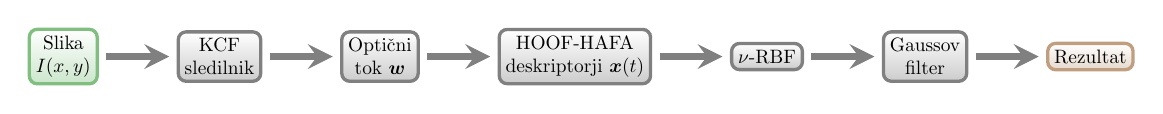
\begin{tikzpicture}
% LAYERS
\pgfdeclarelayer{bg}
\pgfsetlayers{bg,main}
\tikzset{
    between/.style args={#1 and #2}{
         at = ($(#1)!0.5!(#2)$)
    }
}

% NODES
\node (slika) [input] at (0,0) {Slika\\$I(x,y)$};
\node (tracker) [block, right= of slika] {KCF\\sledilnik};
%\node (tarca) [block, right= of tracker] {Področje tarče};

\node (of) [block, right= of tracker] {Optični\\tok $\vec{w}$};
\node (hoof) [block, right= of of] {HOOF-HAFA\\deskriptorji $\vec{x}(t)$};


\node (ucenje) [block, right=of hoof] {\nurbf};
\node (kalman) [block, right= of ucenje] {Gaussov\\filter};


\node (rezultat) [output, right= of kalman] {Rezultat};

% arrows
\draw [arrow] (slika) -- (tracker);
\draw [arrow] (tracker) -- (of);
%\draw [arrow] (tarca) -- (of);
\draw [arrow] (of) -- (hoof);
\draw [arrow] (hoof) -- (ucenje);
\draw [arrow] (ucenje) -- (kalman);
\draw [arrow] (kalman) -- (rezultat);
\end{tikzpicture}}
	\caption[P2OF predikcijska shema]{P2OF predikcijska shema. Uporabljamo jo jo za testiranje modelov z optičnim tokom v 2. fazi.}
	\label{fig:diagram-procesiranja-of-stage2}
\end{figure}


Merjencem smo v P2OF sledili s sledilnikom KCF, ki smo ga nadzorovano reinicializirali vsako minuto. Za izbrano področje slike smo izračunali optični tok. Primer dobljenega optičnega toka je prikazan na sliki~\ref{fig:opticni-tok-stage2}. Sledilo je generiranje HOOF-HAFA deskriptorjev s parametri $N_{HOOF} = 60$ in $N_{HAFA} = 60$. HAFA deskriptorje smo normalizirali z vrednostmi amplitudnih faktorjev $f_A$. %, ki so zbrani v tabeli~\ref{tab:fa-merjenci}.



\begin{figure}[!htb]
	\centering
	\begin{subfigure}[t]{0.45\columnwidth}
		\centering
		\includegraphics[width=0.5\columnwidth, frame]{stage2-lab-of-sv-flo-corrected.png}
		\caption{Stranska slika.}
		\label{fig:stage2-lab-of-sv-flo}
	\end{subfigure}
	~
	\begin{subfigure}[t]{0.45\columnwidth}
		\centering
		\includegraphics[width=0.5\columnwidth, frame]{stage2-lab-of-bv-flo-corrected.png}
		\caption{Hrbtna slika.}
		\label{fig:stage2-lab-of-bv-flo}
	\end{subfigure}
	~
	\begin{subfigure}[t]{0.45\columnwidth}
		\includegraphics[width=\columnwidth]{stage2-lab-sv-of-hist-sl}
		\caption{Histogram stranske slike.}
	\end{subfigure}
	~
	\begin{subfigure}[t]{0.45\columnwidth}
		\includegraphics[width=\columnwidth]{stage2-lab-bv-of-hist-sl}
		\caption{Histogram hrbtne slike.}
	\end{subfigure}
git    \caption[Stranski in hrbtni optični tok ter pripadajoča deskriptorja]{Stranski in hrbtni optični tok ter pripadajoča deskriptorja. Sliki \subref{fig:stage2-lab-of-sv-flo}) in \subref{fig:stage2-lab-of-bv-flo}) sta optična toka detekcije merjencev na sliki~\ref{fig:primer-posnetka-stage2}. V spodnjem levem kotu posamezne slike sta legendi barvnega kodiranja. Na sliki uporabljamo standardno barvno kodiranje, povzeto po~\cite{baker2011database}. Maksimalna amplituda optičnega toka je na sliki  \subref{fig:stage2-lab-of-sv-flo}) znašala \SI{6}{ppf} in na \subref{fig:stage2-lab-of-bv-flo}) \SI{6}{ppf}. Optičnima tokoma pripadata izračunana HOOF-HAFA histograma.}
	\label{fig:opticni-tok-stage2}
\end{figure}


\begin{comment}
\begin{table}[!htb]
	\centering
	\begin{tabular}{l l S[table-format=3.3] | l l S[table-format=3.3]}
		\toprule
		\thead{Pogled} & \thead{Merjenec} & \theadm{f_A} & \thead{Pogled} & \thead{Merjenec} & \theadm{f_A} \\
		\midrule
		\multirow{7}{*}{hrbtni}
		&1&208.557&\multirow{7}{*}{stranski}
		&1&236.985\\	
		&2&179.011&&2&163.957\\
		&4&225.568&&4&196.461\\
		&7&195.133&&7&205.760\\
		&8&209.991&&8&190.253\\
		&9&182.003&&9&178.16\\
		&10&207.002\\
		\bottomrule
	\end{tabular}
	\caption[Faktor amplitud za posamezne merjence pri različnem pogledu]{Faktor amplitud za posamezne merjence pri različnem pogledu.}
	\label{tab:fa-merjenci}
\end{table}
\end{comment}


Procesiranje s prostorskim tokom je za malenkost drugačno. Označili smo ga P2SF. Shematski prikaz procesiranja je prikazan na sliki~\ref{fig:diagram-procesiranja-sf-stage2}.

\begin{figure}[!htb]
	\centering
	\resizebox{\columnwidth}{!}{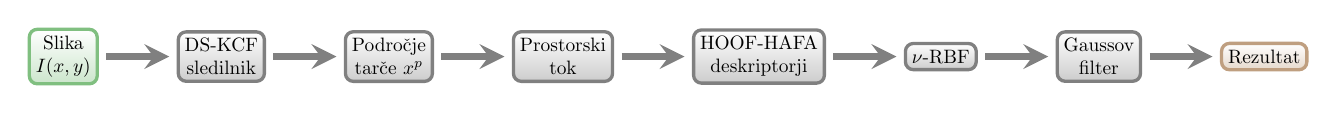
\begin{tikzpicture}
% LAYERS
\pgfdeclarelayer{bg}
\pgfsetlayers{bg,main}
\tikzset{
	between/.style args={#1 and #2}{
		at = ($(#1)!0.5!(#2)$)
	}
}

% NODES
\node (slika) [input] at (0,0) {Slika\\$I(x,y)$};
\node (tracker) [block, right= of slika] {DS-KCF\\sledilnik};
\node (tarca) [block, right= of tracker] {Področje\\ tarče $x^{p}$};

\node (of) [block, right= of tarca] {Prostorski\\ tok};
\node (hoof) [block, right= of of] {HOOF-HAFA\\deskriptorji};


\node (ucenje) [block, right=of hoof] {\nurbf};
\node (kalman) [block, right= of ucenje] {Gaussov\\ filter};


\node (rezultat) [output, right= of kalman] {Rezultat};

% arrows
\draw [arrow] (slika) -- (tracker);
\draw [arrow] (tracker) -- (tarca);
\draw [arrow] (tarca) -- (of);
\draw [arrow] (of) -- (hoof);
\draw [arrow] (hoof) -- (ucenje);
\draw [arrow] (ucenje) -- (kalman);
\draw [arrow] (kalman) -- (rezultat);
\end{tikzpicture}}
	\caption[P2SF predikcijska shema]{P2SF predikcijska shema. Uporabljamo jo za testiranje modelov s prostorskim tokom v fazi 2.}
	\label{fig:diagram-procesiranja-sf-stage2}
\end{figure}

Merjencem smo v P2SF sledili s sledilnikom DS-KCF, ki smo ga nadzorovano reinicializirali vsako minuto. Izbranim področjem smo izračunali prostorski tok. Primer dobljenega optičnega toka je prikazan na sliki~\ref{fig:prostorski-tok-stage2}. Sledilo je generiranje HOOF-HAFA deskriptorjev po postopku P2OF, le da HAFA deskriptorjev nismo normalizirali, ker smo histograme pridobili iz podatkov z metričnimi enotami. 


\begin{figure}[!htb]
	\centering
	\begin{subfigure}[t]{0.45\columnwidth}
		\centering
		\includegraphics[width=\columnwidth, frame]{stage2-lab-sf-sv-pdflow-corrected.jpg}
		\caption{Stranska slika.}
	\end{subfigure}
	~
	\begin{subfigure}[t]{0.45\columnwidth}
		\centering
		\includegraphics[width=\columnwidth, frame]{stage2-lab-sf-bv-pdflow-corrected.jpg}
		\caption{Hrbtna slika.}
	\end{subfigure}
	%~
	%\begin{subfigure}[t]{0.45\columnwidth}
	%	\centering
	%	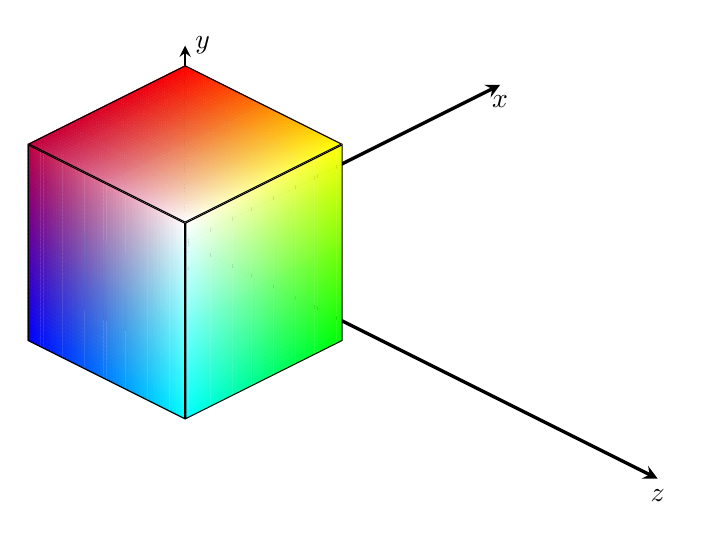
\begin{tikzpicture}%[tdplot_main_coords, scale=0.5]
[x={(0.8cm,0.4cm)}, y={(0cm,1cm)}, z={(0.8cm,-0.4cm)}, scale=0.5]

\pgfmathtruncatemacro{\Divisions}{50};
\pgfmathsetmacro{\Cube}{5};
%\definecolor{mypurple}{RGB}{255,0,255};

	% Coordinate system
    \coordinate (O) at (0,0,0);
    \coordinate (oo) at (0,0,5);
    \coordinate (y) at (0,5,0);
    \coordinate (z) at (0,0,15);
    \coordinate (x) at (10,0,0);
    \draw [axis, thick] (O) -- (y) node [right] {$y$};
    \draw [axis] (O) -- (z) node [below] {$z$};
    \draw [axis] (O) -- (x) node [below] {$x$};
    \node (izhodisce) [below] at (O) {$\vec{O}$};
   
    
    \begin{scope}[canvas is yz plane at x=-\Cube/2]
    \shade[lower right=purple, lower left=blue, upper right=white, upper left=cyan] (-1,-1) rectangle (1,1);
    \clip (-\Cube/2,-\Cube/2) rectangle (\Cube/2,\Cube/2);
    \colorlet{BL}[RGB]{blue}
    \colorlet{BR}[RGB]{purple}
    \colorlet{TL}[RGB]{cyan}
    \colorlet{TR}[RGB]{white}
    \foreach \x in {1,...,\Divisions}
    {   \pgfmathtruncatemacro{\px}{(\x-1)/(\Divisions-1)*100}
    	\colorlet{B}[RGB]{BR!\px!BL}
    	\colorlet{T}[RGB]{TR!\px!TL}
    	\foreach \y in {1,...,\Divisions}
    	{   \pgfmathtruncatemacro{\py}{(\y-1)/(\Divisions-1)*100}
    		\fill[T!\py!B] ({-\Cube/2+\Cube*(\x-1)/\Divisions},{-\Cube/2+\Cube*(\y-1)/\Divisions}) rectangle ({-\Cube/2+\Cube*(\x+0.1)/\Divisions},{-\Cube/2+\Cube*(\y+0.1)/\Divisions});
    	}
    }
    \draw[thick] (-\Cube/2,-\Cube/2) rectangle (\Cube/2,\Cube/2);
    \end{scope}
    
    \begin{scope}[canvas is xz plane at y=\Cube/2]
    \clip (-\Cube/2,-\Cube/2) rectangle (\Cube/2,\Cube/2);
    \colorlet{BL}[RGB]{purple}
    \colorlet{BR}[RGB]{red}
    \colorlet{TL}[RGB]{white}
    \colorlet{TR}[RGB]{yellow}
    \foreach \x in {1,...,\Divisions}
    {   \pgfmathtruncatemacro{\px}{(\x-1)/(\Divisions-1)*100}
    	\colorlet{B}[RGB]{BR!\px!BL}
    	\colorlet{T}[RGB]{TR!\px!TL}
    	\foreach \y in {1,...,\Divisions}
    	{   \pgfmathtruncatemacro{\py}{(\y-1)/(\Divisions-1)*100}
    		\fill[T!\py!B] ({-\Cube/2+\Cube*(\x-1)/\Divisions},{-\Cube/2+\Cube*(\y-1)/\Divisions}) rectangle ({-\Cube/2+\Cube*(\x+0.1)/\Divisions},{-\Cube/2+\Cube*(\y+0.1)/\Divisions});
    	}
    }
    \draw[thick] (-\Cube/2,-\Cube/2) rectangle (\Cube/2,\Cube/2);
    \end{scope}
    
    \begin{scope}[canvas is xy plane at z=\Cube/2]
    \clip (-\Cube/2,-\Cube/2) rectangle (\Cube/2,\Cube/2);
    \colorlet{BL}[RGB]{cyan}
    \colorlet{BR}[RGB]{green}
    \colorlet{TL}[RGB]{white}
    \colorlet{TR}[RGB]{yellow}
    \foreach \x in {1,...,\Divisions}
    {   \pgfmathtruncatemacro{\px}{(\x-1)/(\Divisions-1)*100}
    	\colorlet{B}[RGB]{BR!\px!BL}
    	\colorlet{T}[RGB]{TR!\px!TL}
    	\foreach \y in {1,...,\Divisions}
    	{   \pgfmathtruncatemacro{\py}{(\y-1)/(\Divisions-1)*100}
    		\fill[T!\py!B] ({-\Cube/2+\Cube*(\x-1)/\Divisions},{-\Cube/2+\Cube*(\y-1)/\Divisions}) rectangle ({-\Cube/2+\Cube*(\x+0.1)/\Divisions},{-\Cube/2+\Cube*(\y+0.1)/\Divisions});
    	}
    }
    \draw[thick] (-\Cube/2,-\Cube/2) rectangle (\Cube/2,\Cube/2);
    \end{scope}
	    
\end{tikzpicture}
	%	\caption{Hrbtna slika.}
	%\end{subfigure}
	\caption[Prostorski tok za sliki~\ref{fig:primer-posnetka-stage2}]{Prostorski tok za sliki~\ref{fig:primer-posnetka-stage2}. Slike smo pridobili s programom \texttt{Scene-Flow-Impair} avtorja~\cite{jaimez2015primal}, ki smo ga prilagodili za Kinect V2 kamero. Sliki sta 8-bit RGB sliki. Amplitude hitrosti v posameznih oseh so normirane in normalizirane na intervalu $[0,255]$. Kanal B predstavlja komponento $\mu_x$, kanal G $\mu_y$, ter kanal R $\mu_z$ prostorskega toka $\vec{\mu}$. Beli slikovni elementi so neveljavni (ne vsebujejo podatka o globini).}
	\label{fig:stage2-lab-sf-pd}
\end{figure}

\begin{figure}[!htb]
	\centering
	\begin{subfigure}[t]{0.45\columnwidth}
		\centering
		\includegraphics[width=0.5\columnwidth, frame]{./Slike/stage2-lab-sf-sv-flo-corrected.png}
		\caption{stranska slika}
		\label{fig:stage2-lab-sf-sv-flo}
	\end{subfigure}
	~
	\begin{subfigure}[t]{0.45\columnwidth}
		\centering
		\includegraphics[width=0.5\columnwidth, frame]{./Slike/stage2-lab-sf-bv-flo-corrected.png}
		\caption{hrbtna slika}
		\label{fig:stage2-lab-sf-bv-flo}
	\end{subfigure}
	~
	\begin{subfigure}[t]{0.45\columnwidth}
		\includegraphics[width=\columnwidth]{stage2-lab-sv-sf-hist-sl}
		\caption{Histogram stranske slike.}
	\end{subfigure}
	~
	\begin{subfigure}[t]{0.45\columnwidth}
		\includegraphics[width=\columnwidth]{stage2-lab-bv-sf-hist-sl}
		\caption{Histogram hrbtne slike.}
	\end{subfigure}
	\caption[Projekcije prostorskih tokov na slikovno ravnino]{Projekcija prostorskih tokov na slikovno ravnino. Gre za prostorska toka detekcije merjencev na sliki~\ref{fig:primer-posnetka-stage2}. V spodnjem levem kotu posamezne slike sta legendi barvnega kodiranja. Na sliki uporabljamo standardno barvno kodiranje, povzeto po~\cite{baker2011database}. Maksimalna amplituda prostorskega toka je na sliki  \subref{fig:stage2-lab-sf-sv-flo}) znašala \SI{10.4}{\m\per\s} in na \subref{fig:stage2-lab-sf-bv-flo}) \SI{9.4}{\m\per\s}. Projekcijama prostorskega toka pripadata izračunana HOOF-HAFA histograma.}
	\label{fig:prostorski-tok-stage2}
\end{figure}



Modele obeh postopkov (P2OF in P2SF) smo učili s postopkom \nurbf, kjer smo za Gaussov filter uporabili $\sigma=5$ in za največje število podpornih vektorjev $\numax =0.5$ (\SI{50}{\%} podpornih vektorjev). Podobno kot v eksperimentih 1. faze smo tudi tu naučili \num{6} elementarnih modelov, in sicer: \textit{eem} modele, ki predvidevajo porabo energije v \si{\kcal\per\min}, \textit{sv} modele za stransko kamero in \textit{bv} modele za hrbtno kamero. %ter \textit{lag} modele z upoštevanjem časovne zakasnitve.

%Vse tipe eksperimentov smo križno testirali glede na enak tip eksperimenta, le z drugim zornim kotom kamere. Uporabljen zorni kot kamere za križno testiranje je v imenih modelov zapisan v oklepajih.  

Rezultate smo filtrirali z Gaussovim jedrom $\sigma=5$. Modele smo testirali po treh različnih protokolih iz razlogov, ki jih izrecno navajamo. %S prvim protokolom smo preverjali neodvisnost od časovnega povečevanja porabe, z drugim pa ravno obratno. S tretjim protokolom smo želeli pokazati delovanje posplošenega modela na različnih merjencih.


\paragraph{Protokol 1.}
Za testne vzorce vzamemo vsak 3. vzorec fiziološkega parametra in slike iz posameznega posnetka. Ostale vzorce uporabimo pri učenju. Rezultate vseh 6 meritev povprečimo. Na tak način smo poskušali učiti modele, ki so neodvisni od časovnega povečevanja utrujenost.

\paragraph{Protokol 2.}
Za učne vzorce izberemo prvih \SI{70}{\%} vzorce in za testne naslednjih \SI{30}{\%}. Rezultate vseh 6 meritev povprečimo.

\paragraph{Protokol 3.}
Uporabimo protokol 1, pri čemer učimo na prvih štirih meritvah in testiramo na zadnjih dveh. Rezultatov ne povprečimo. Na ta način smo proučili možnost posplošitve naučenih modelov za uporabo na merjencih, ki niso bili vključeni v učenje.

\begin{comment}
\subsubsection{Določitev zakasnitve fiziološkega odziva}
Določitve zakasnitve fiziološkega odziva smo se, glede na eksperimente 1. faze, tu lotili nekoliko drugače. Na podlagi protokola izvajanja meritev, smo pridobili podatke eno minutnega mirovanja posameznega merjenca z vzorčno frekvenco \SI{0.2}{\hertz}. Kljub temu, da je signal v stacionarnem stanju, je nihajoč zaradi narave fiziologije. Signal mirovanja smo interpolirali na vzorčno frekvenco \SI{1}{\hertz}. Določili smo mu srednjo vrednost in vrednost treh standardnih odklonov. S tem smo dobili interval nedoločenosti, v katerem ne moremo določiti ali je pri spremembi amplitude signala prišlo zaradi fizioloških dejavnikov ali zaradi dejanskega odziva na vzbujalni signal. 

Na podlagi slik~\ref{fig:lag-estimation-stage2}, smo zakasnitev za posamezno meritev določili kot časovni interval od trenutka spremembe hitrosti tekalne steze do trenutka, ko je bila vrednost fiziološkega parametra prvič nad intervalom nedoločenosti. Zakasnitev smo, zaradi treh standardnih odklonov, lahko določili s \SI{99.73}{\%} zagotovostjo za posameznega merjenca. Zakasnitve vseh merjencev smo povprečili in dobili vrednost \SI{26}{\s} za energijsko porabo.

\begin{figure}[!htbp]
	\centering
	\begin{subfigure}[t]{0.45\columnwidth}
		\includegraphics[width=\columnwidth]{stage2-lag-estimation-1-eem-sl}
		\caption{Zakasnitev za subjekt 1.}
		\label{fig:lag-estimation-1-eem}
	\end{subfigure}
	~
	\begin{subfigure}[t]{0.45\columnwidth}
		\includegraphics[width=\columnwidth]{stage2-lag-estimation-2-eem-sl}
		\caption{Zakasnitev za subjekt 2.}
		\label{fig:lag-estimation-2-eem}
	\end{subfigure}
	~
	\begin{subfigure}[t]{0.45\columnwidth}
		\includegraphics[width=\columnwidth]{stage2-lag-estimation-3-eem-sl}
		\caption{Zakasnitev za subjekt 3.}
		\label{fig:lag-estimation-3-eem}
	\end{subfigure}
	~
	\begin{subfigure}[t]{0.45\columnwidth}
		\includegraphics[width=\columnwidth]{stage2-lag-estimation-4-eem-sl}
		\caption{Zakasnitev za subjekt 4.}
		\label{fig:lag-estimation-4-eem}
	\end{subfigure}
	~
	\begin{subfigure}[t]{0.45\columnwidth}
		\includegraphics[width=\columnwidth]{stage2-lag-estimation-5-eem-sl}
		\caption{Zakasnitev za subjekt 5.}
		\label{fig:lag-estimation-5-eem}
	\end{subfigure}
	~
	\begin{subfigure}[t]{0.45\columnwidth}
		\includegraphics[width=\columnwidth]{stage2-lag-estimation-6-eem-sl}
		\caption{Zakasnitev za subjekt 6.}
		\label{fig:lag-estimation-6-eem}
	\end{subfigure}
	\caption[Prikaz določitve zakasnitve za posameznega merjenca]{Prikaz določitve zakasnitve za posameznega merjenca. Zakasnitev za posamezno meritev smo določili kot časovni interval od trenutka spremembe hitrosti tekalne steze do trenutka, ko je bila vrednost fiziološkega parametra prvič nad intervalom nedoločenosti. Interval nedoločenosti je prikazan z zelenimi horizontalnimi linijami. Rumeni vzorci so vzorci enominutnega mirovanja. Sledijo modri vzorci pri hoji na tekalni stezi s hitrostjo \SI{5}{\km\per\hour}. Spremenba hitrosti tekalne steze je prikazana z rdečim signalom.}
	\label{fig:lag-estimation-stage2}
\end{figure}
\end{comment}









\subsection{Terenski eksperimenti}
Šest igralcev je igralo tri squash igre. V vsaki igri sta bila dva seta. Igre so trajale \SI{16}{\min}, \SI{14}{\min} in \SI{11}{\min}. Uporabili smo P2OF in P2SF procesiranje z nadzorovano reinicializacijo sledilnikov vsake \SI{2}{\s}. Delovanje sledilnikov lahko vidimo na sliki~\ref{fig:stage2-field-tracked}. Pripadajoči optični in prostorski tok sta prikazana na sliki~\ref{fig:stage2-field-sfof}. Na sliki~\ref{fig:stage2-field-hist} sta prikazana pripadajoča histograma.

\begin{figure}[!htb]
	\centering
	\begin{subfigure}{0.45\columnwidth}
		\centering
		\includegraphics[width=\columnwidth]{stage2-field-of-left-tracked.png}
		\caption{KCF sledilnik}
	\end{subfigure}
	~
	\begin{subfigure}{0.45\columnwidth}
		\centering
		\includegraphics[width=\columnwidth]{stage2-field-sf-left-tracked.png}
		\caption{DS-KCF sledilnik.}
	\end{subfigure}
	\caption[Predstavitev delovanja KCF in DS-KCF sledilnikov]{Predstavitev delovanja KCF in DS-KCF sledilnikov za terenske eksperimente. Za primerjavo sledilnikov sta prikazani 120. sliki leve kamere prvega seta 2. igre za merjenca SUBJ9. Zelena okvirja prikazujeta detektirani področji za posamezen sledilnik. Opazimo, da sta področji različni.}
	\label{fig:stage2-field-tracked}
\end{figure}



\begin{figure}[!htb]
	\centering
	\begin{subfigure}[t]{0.3\columnwidth}
		\centering
		\includegraphics[width=\columnwidth, frame]{./Slike/stage2-field-of-svbv-flo-corrected.png}
		\caption{Optični tok.}
		\label{fig:stage2-field-of}
	\end{subfigure}
	~
	\begin{subfigure}[t]{0.3\columnwidth}
		\centering
		\includegraphics[width=\columnwidth, frame]{./Slike/stage2-field-sf-svbv-flo-corrected.png}
		\caption{Projekcija prostorskega toka.}
		\label{fig:stage2-field-pd}
	\end{subfigure}
	~
	\begin{subfigure}[t]{0.3\columnwidth}
		\centering
		\includegraphics[width=\columnwidth, frame]{./Slike/stage2-field-sf-pd-tr-corrected.jpg}
		\caption{Prostorski tok.}
	\end{subfigure}
	\caption[Optični tok, prostorski tok in njegova projekcija]{Optični tok, prostorski tok in njegova projekcija na slikovno ravnino. V spodnjem levem kotu optičnega tok in projekcije prostorskega toka sta legendi barvnega kodiranja. Uporabljamo standardno barvno kodiranje, povzeto po~\cite{baker2011database}. Maksimalna amplituda optičnega toka na sliki  \subref{fig:stage2-field-of}) je  \SI{10}{ppf}. Maksimalna amplituda projekcije prostorskega toka je \SI{13.7}{\m\per\s}. Sliko prostorskega toka \subref{fig:stage2-field-pd}) smo pridobili s programom \texttt{Scene-Flow-Impair} avtorja~\cite{jaimez2015primal}, ki smo ga prilagodili za Kinect V2 kamero. Slika je 8-bitna RGB. Amplitude hitrosti v posameznih oseh so normirane in normalizirane na intervalu $[0,255]$. Kanal B predstavlja komponento $\mu_x$, kanal G $\mu_y$, ter kanal R $\mu_z$ prostorskega toka $\vec{\mu}$. Beli slikovni elementi so neveljavni (ne vsebujejo podatka o globini).}
	\label{fig:stage2-field-sfof}
\end{figure}



\begin{figure}[!htb]
	\centering
	\begin{subfigure}[t]{0.45\columnwidth}
		\includegraphics[width=\columnwidth]{stage2-field-bv-of-hist-sl}
		\caption{Histogram optičnega toka.}
	\end{subfigure}
	~
	\begin{subfigure}[t]{0.45\columnwidth}
		\includegraphics[width=\columnwidth]{stage2-field-bv-sf-hist-sl}
		\caption{Histogram prostorskega toka.}
	\end{subfigure}
	\caption[Histograma optičnega in projekcije prostorskega toka]{Histograma optičnega in projekcije prostorskega toka. Histogram za optični tok smo dobili iz slike~\ref{fig:stage2-field-sfof}\subref{fig:stage2-field-of}). Histogram projekcije prostorskega toka smo dobili iz slike~\ref{fig:stage2-field-sfof}\subref{fig:stage2-field-pd}}
	\label{fig:stage2-field-hist}
\end{figure}

\begin{comment}
\begin{figure}[!htb]
	\centering
	\begin{subfigure}[t]{0.45\columnwidth}
		\includegraphics[width=1.2\columnwidth]{stage2-field-left-depth-sl}
		\caption{Stranska slika.}
	\end{subfigure}
	~
	\begin{subfigure}[t]{0.45\columnwidth}
		\includegraphics[width=1.2\columnwidth]{stage2-field-right-depth-sl}
		\caption{Hrbtna slika.}
	\end{subfigure}
	\caption[Stranska in hrbtna globinska slika pri terenskih testih 2. faze]{Stranska in hrbtna globinska slika pri terenskih testih 2. faze.}
	\label{fig:stage2-field-of-depth}
\end{figure}
\end{comment}



\subsubsection{Pridobivanje podatkov.}
\paragraph{Fiziolo\v{ski} parametri.}
Fiziološke parametre smo pridobili s pomočjo prenosnega sistema za direktno ergospirometrijo tipa ``breath  by breath'' Cosmed K4B2. Sistem je prikazan na sliki~\ref{fig:maske}. Frekvenca vzorčenja se je spreminjala, v povprečju pa je znašala \SI{0.5}{\hertz}. S testom smo pridobili podatke energijske porabe šestih različnih merjencev (SUBJ1, SUBJ2, SUBJ7, SUBJ8, SUBJ9 in SUBJ10).


\begin{figure}[!htb]
	\centering
	\includegraphics[width=0.4\columnwidth]{./Slike/squash-maske-corrected.jpg}	
	\caption[Prenosni sistem za direktno ergospirometrijo]{Prenosni sistem za direktno ergospirometrijo tipa ``breath  by breath'' Cosmed K4B2.}
	\label{fig:maske}
\end{figure}

\paragraph{Video posnetki.}
Igrišče smo snemali z dvema Microsoft Xbox Kinect V2 kamerama, ki sta bili oddaljeni ena od druge za približno \SI{2}{m}. Vsaka kamera je pokrivala svojo polovico igrišča. Razdalja od tal je znašala približno \SI{3}{m}. Kameri sta bili tako pozicionirani nad zaščitnim steklom. S tem nismo dobili odbojev laserskih žarkov, ki so namenjeni za pridobivanje globinske slike. Kot $\theta$ (rotacija okoli x osi) je bil približno $30\stopinj$ tako, da so kamere pokrivale prvo polovico igrišča do linije serviranja. Postavitev kamer je prikazana na sliki~\ref{fig:field-postavitev-kamer}.

\begin{figure}[!htb]
	\centering
	\includegraphics[width=0.6\columnwidth]{squash-postavitev-corrected.jpg}	
	\caption[Postavitev Kinect kamer pri terenskih testih 2. faze]{Postavitev Kinect kamer pri terenskih testih 2. faze.}
	\label{fig:field-postavitev-kamer}
\end{figure}


Pridobili smo barvne RGB in globinske DEPTH slike. Snemali smo v ločljivosti $512 \times 424$. Hitrost posnetkov je znašala \SI{30}{fps}. Kameri smo časovno sinhronizirali po NTP protokolu.



\paragraph{Protokol meritve.}
Posamezno igro smo pričeli s 5 minutnim ogrevalnim tekom. Sledilo je igranje na dva seta do 10 dobljenih točk z upoštevanjem dveh točk razlike. Med setoma so igralci počivali 2 minute. Ogrevanja in počivanja s kamerami nismo merili. Seta posamezne igre smo združili v en posnetek.


\chapter{Rezultati}\label{sec:rezultati}
All energy consumption and heart rate models were validated on previously described test samples. For comparison between the different models we have chosen validation measures: correlation coefficient (CORR), relative absolute error (RAE) and root relative square error (RRSE) \cite{witten2005data}.The higher the value of the CORR the better, with RAE and RRSE is other way around.

% Dodati moram da sem 8 initial modelov potem cross teste delal
Models were also evaluated with cross testing. This testing was done only by the type of input data---side-view or back-view. \textit{sv} models, that were made with learning samples from side-view camera were first tested with testing samples from side-view camera and then with back-view camera. Hereafter tests with input data from side-view camera are marked with \textit{sv} in brackets and tests with input data from back-view camera are marked with \textit{bv} in brackets.



















\section{Eksperimenti 1. faze}


\subsection{Preliminarni testi}

\subsubsection{Optimizacija HOOF deskriptorjev}\label{sec:rezultati-optimizacija-hoof}
Parameter $N_{HOOF}$ smo določili na podlagi rezultatov evaluacije v tabeli \ref{tab:nhoof} in grafov korelacije med referenčnimi podatki in predikcijo \ref{fig:corr-hoof}.

V tabeli \ref{tab:nhoof} lahko vidimo, da se povečevanjem števila stolpcev rezultati bistveno ne razlikujejo. Najbojlši rezultate nam sicer daje $120$ stolpcev, vendar pa smo za potrebe naše metode uporabili $N_{HOOF}=60$, ki je ravno tako dal zadovoljive rezultate. S takim številom smo zagotovili dobro delovanje glede na minimalno vrednost, še vseeno pa ne gre za tako veliko število, ko bi do izraza prišle amplitude šumnih vektorjev.

\begin{table}[!htbp]
	\centering
	\begin{tabular}{S[table-format=2.0] S[table-format=1.3] S[table-format=1.3] S[table-format=1.3] S[table-format=2.2]}
		\toprule
		\thead{$\mathbf{N_{HOOF}}$} & \thead{$\mathbf{r}$} & \thead{RAE} & \thead{RRSE} & \thead{nSV [\%]}\\
		\midrule%nSV
		30 & 0.978 & 0.296 & 0.304 & \boldentry{2}{2}{62.81}\\%18089
		\boldentry{2}{0}{60} & 0.980 & 0.277 & 0.289 & 81.21\\%23388
		120 & \boldentry{1}{2}{0.983} & \boldentry{1}{3}{0.261} & \boldentry{1}{3}{0.273} & 74.39\\%21424
		160 & 0.982 & 0.272 & 0.284 & 71.68\\%20644
		\bottomrule
	\end{tabular}
	\caption[Rezultati evaluacije modelov z različnim $N_{HOOF}$]{Rezultati evaluacije modelov z različnim številom stolpcev $N_{HOOF}$ HOOF deskriptorja. Optimalni rezultati so odebeljeni. Kljub dobrim rezultatom modela z $N_{HOOF}=120$ smo izbrali $N_{HOOF}=60$, ker nanj šum manj vpliva.}
	\label{tab:nhoof}
\end{table}

\begin{figure}[!htbp]
	\centering
	\begin{subfigure}[t]{0.45\columnwidth}
		\includegraphics[width=\columnwidth]{corr-hoof-30-sl}
		\caption{Korelacija $N_{HOOF}=30$.}
		\label{fig:corr-hoof-30}
	\end{subfigure}
	~
	\begin{subfigure}[t]{0.45\columnwidth}
		\includegraphics[width=\columnwidth]{corr-hoof-60-sl}
		\caption{Korelacija $N_{HOOF}=60$.}
		\label{fig:corr-hoof-60}
	\end{subfigure}
	~
	\begin{subfigure}[b]{0.45\columnwidth}
		\includegraphics[width=\columnwidth]{corr-hoof-120-sl}
		\caption{Korelacija $N_{HOOF}=120$.}
		\label{fig:corr-hoof-120}
	\end{subfigure}
	~
	\begin{subfigure}[b]{0.45\columnwidth}
		\includegraphics[width=\columnwidth]{corr-hoof-160-sl}
		\caption{Korelacija $N_{HOOF}=160$.}
		\label{fig:corr-hoof-160}
	\end{subfigure}
	\caption[Grafi korelacij modelov z različnim $N_{HOOF}$]{Grafi korelacij modelov z različnim številom stolpcev $N_{HOOF}$ HOOF deskriptorja. Rezultati so si zelo podobni.}
	\label{fig:corr-hoof}
\end{figure}












\subsubsection{Optimizacija HAFA deskriptorjev}\label{sec:rezultati-optimizacija-hafa}
Parameter $N_{HAFA}$ smo določili na podlagi rezultatov evaluacije v tabeli \ref{tab:nhafa} in grafov korelacije med referenčnimi podatki in predikcijo \ref{fig:corr-hafa}.

\begin{table}[!htbp]
	\centering
	\begin{tabular}{S[table-format=2.0] S[table-format=1.3] S[table-format=1.3] S[table-format=1.3] S[table-format=2.2]}
		\toprule
		\thead{$\mathbf{N_{HAFA}}$} & \thead{$\mathbf{r}$} & \thead{RAE} & \thead{RRSE} & \thead{nSV [\%]}\\
		\midrule%nSV
		30 & 0.984 & 0.213 & 0.231 & 62.08 \\%17879/28799
		\boldentry{2}{0}{60} & \boldentry{1}{3}{0.984} & \boldentry{1}{3}{0.211} & \boldentry{1}{3}{0.228} & \boldentry{2}{2}{62.60} \\%18028
		120 & 0.984 & 0.211 & 0.228 & 62.63 \\%18037
		160 & 0.984 & 0.211 & 0.228 & 62.63 \\%18037
		\bottomrule
	\end{tabular}
	\caption[Rezultati evaluacije modelov z različnim $N_{HAFA}$]{Rezultati evaluacije modelov z različnim številom stolpcev $N_{HAFA}$ HAFA deskriptorja. Optimalni rezultati so odebeljeni.}
	\label{tab:nhafa}
\end{table}

V tabeli \ref{tab:nhafa} lahko vidimo, da so rezultati praktično enaki. Za našo metodo smo izbrali $N_{HAFA}=60$, kar v grobem predstavlja $60$ različnih hitrosti z maksimalno amplitudo \SI{60}{px.f^{-1}}.

\begin{figure}[!htbp]
	\centering
	\begin{subfigure}[t]{0.45\columnwidth}
		\includegraphics[width=\columnwidth]{corr-hafa-30-sl}
		\caption{Korelacija $N_{HAFA}=30$.}
		\label{fig:corr-hafa-30}
	\end{subfigure}
	~
	\begin{subfigure}[t]{0.45\columnwidth}
		\includegraphics[width=\columnwidth]{corr-hafa-60-sl}
		\caption{Korelacija $N_{HAFA}=60$.}
		\label{fig:corr-hafa-60}
	\end{subfigure}
	~
	\begin{subfigure}[b]{0.45\columnwidth}
		\includegraphics[width=\columnwidth]{corr-hafa-120-sl}
		\caption{Korelacija $N_{HAFA}=120$.}
		\label{fig:corr-hafa-120}
	\end{subfigure}
	~
	\begin{subfigure}[b]{0.45\columnwidth}
		\includegraphics[width=\columnwidth]{corr-hafa-160-sl}
		\caption{Korelacija $N_{HAFA}=160$.}
		\label{fig:corr-hafa-160}
	\end{subfigure}
	\caption[Grafi korelacij modelov z različnim $N_{HAFA}$]{Grafi korelacij modelov z različnim številom stolpcev $N_{HAFA}$ HAFA deskriptorja. Rezultati so si zelo podobni.}
	\label{fig:corr-hafa}
\end{figure}











\subsubsection{Razširitev HOOF deskriptorja}\label{sec:rezultati-razsiritev-hoof}

\begin{table}[!htbp]
	\centering
	\begin{tabular}{l S[table-format=1.3] S[table-format=1.3] S[table-format=1.3] S[table-format=2.2]}
		\toprule
		\textbf{Deskriptor} & \thead{$\mathbf{r}$} & \thead{RAE} & \thead{RRSE} & \thead{nSV [\%]}\\
		\midrule%nSV
		HOOF & 0.992 & 0.336 & 0.317 & \boldentry{2}{2}{82.34} \\%2187/2656
		\textbf{HOOF-HAFA} & \boldentry{1}{3}{0.991} & \boldentry{1}{3}{0.157} & \boldentry{1}{3}{0.205} & 89.53 \\%2378
		\bottomrule
	\end{tabular}
	\caption[Rezultati evaluacije modelov z različnim deskriptorjem]{Rezultati evaluacije modelov z različnim deskriptorjem. Optimalni rezultati so odebeljeni. Vidimo lahko, da se bolje odnese razširjeni deskriptor HOOF-HAFA, čeprav model uporablja več podpornih vektorjev. }
	\label{tab:izbira}
\end{table}



\begin{figure}[!htbp]
	\centering
	\begin{subfigure}[t]{0.45\columnwidth}
		\includegraphics[width=\columnwidth]{corr-hoof-sl}
		\caption{Korelacija $N_{HOOF}=60$.}
		\label{fig:izbira-hoof}
	\end{subfigure}
	~
	\begin{subfigure}[t]{0.45\columnwidth}
		\includegraphics[width=\columnwidth]{corr-hoof-hafa-sl}
		\caption{Korelacija $N_{HOOF}=60$,\\$N_{HAFA}=60$.}
		\label{fig:izbira-hoofhafa}
	\end{subfigure}
	\caption[Primerjava modelov s HOOF in HOOF-HAFA deskriptorji]{Primerjava grafov korelacij modelov z različnimi deskriptorji. Model \subref{fig:izbira-hoof}) smo naučili s HOOF deskriptorjem. Model \subref{fig:izbira-hoofhafa}) smo naučili s HOOF in HAFA deskriptorjem. Posamezen vzorec je tako vseboval $120$ značilk. Pri primerjavi korelacije lahko opazimo vidno razliko. Model \subref{fig:izbira-hoofhafa}) dokazuje, da je razširjeni deskriptor boljši.}
	\label{fig:izbira}
\end{figure}




















\subsubsection{Sledilniki za optični tok} \label{sec:rezultati-sledilnikov-za-opticni-tok}


Rezultati testiranja so prikazani v tabeli \ref{tab:region-overlap}. Za izbrane sledilnike smo določili povprečje prekrivanja področja za posamezen posnetek. V tretjem stolpcu je predstavljeno povprečje prekrivanja glede na oba posnetka. Najboljši rezultati so odebeljeni. Po tabeli \ref{tab:region-overlap} se za posnetek \textit{handball1} najbolje izkaže CORR sledilnik. Za posnetek \textit{handball2} smo dobili najboljše rezultate pri sledilniku OPENCV-TLD. V povprečju se najbolje izkaže sledilnik CORR.




\begin{table}[!htbp]
	\centering
	\begin{tabular}{l S[table-format=1.3] S[table-format=1.3] S[table-format=1.3]}
		\toprule
		\textbf{Sledilnik} & \thead{$\mathbf{\Phi(\mathrm{handball1})}$} & \thead{$\mathbf{\Phi(\mathrm{handball2})}$} & \thead{$\mathbf{\overline{\Phi}}$}  \\
		\midrule%nSV
		NEBEHAY-TLD & 0.035 & 0.130 & 0.083 \\
		CCV-TLD & 0.117 & 0 & 0.117 \\
		OPENCV-TLD & 0.002 & \boldentry{1}{3}{0.178} & 0.09 \\
		CORR & \boldentry{1}{3}{0.214} & 0.160 & \boldentry{1}{3}{0.187} \\
		\textbf{KCF} & {0.161} & {0.166} & {0.164} \\
		\bottomrule
	\end{tabular}
	\caption[Povprečje prekrivanja področja za posamezen sledilnik]{Povprečje prekrivanja področja za posamezen sledilnik in posnetek. V tretjem stolpcu je predstavljeno povprečje prekrivanja glede na oba posnetka. Najboljši rezultati so odebeljeni. Po tabeli \ref{tab:region-overlap} se za posnetek \textit{handball1} najbolje izkaže CORR sledilnik. Za posnetek \textit{handball2} smo dobili najboljše rezultate pri sledilniku OPENCV-TLD. V povprečju se najbolje izkaže sledilnik CORR.}
	\label{tab:region-overlap}
\end{table}


Na sliki \ref{fig:tracker-visual} lahko vidimo primer delovanja sledilnikov za oba posnetka. Referenčni igralec, ki mu morajo slediti ima rumeno majico. Za posnetek \textit{handball1} je predstavljena 15. slika, za posnetek \textit{handball2} pa 111. slika. Rezultati v tabeli \ref{tab:region-overlap} se skladajo z opažanji na sliki \ref{fig:tracker-visual}.

\begin{figure}[!htbp]
	\centering
	
	\begin{subfigure}[t]{0.45\columnwidth}
		\includegraphics[width=\columnwidth]{handball1-example.png}
		\caption{15. slika posnetka \textit{handball1}.}
		\label{fig:handball1}
	\end{subfigure}
	~
	\begin{subfigure}[t]{0.45\columnwidth}
		\includegraphics[width=\columnwidth]{/handball2-example.png}
		\caption{111. slika posnetka \textit{handball2}.}
		\label{fig:handball2}
	\end{subfigure}  
	\caption[Primer delovanja sledilnikov za \textit{handball} posnetke]{Primer delovanja sledilnikov za \textit{handball} posnetke. Referenčni igralec, ki mu morajo slediti ima rumeno majico. }
	\label{fig:tracker-visual}
\end{figure}




Čeprav smo z mero določili, da se je najbolje izkazal sledilnik CORR, se je pri hitri vizualni oceni sledenja na izsekih posnetka \cite{squashtv2014squash} izkazalo, da najbolje deluje sledilnik KCF. Primer boljšega delovanja KCF sledilnika je slika \ref{fig:squash-tracker-visual}, kjer sledimo modremu igralcu. Na isti sliki posnetka je KCF algoritem našel modrega igralca, medtem ko ga je CORR algoritem zamenjal z drugim igralcem. 



\begin{figure}[!htbp]
	\centering
	\includegraphics[width=0.6\columnwidth]{preliminary-tracker-squash.png}
	\caption{}
	\caption[Primer delovanja sledilnikov za squash posnetek]{Primer delovanja sledilnikov za squash posnetek. Gre za 41. sliko posnetka \cite{squashtv2014squash}, pri čemer smo uporabili KCF in CORR algoritem. Sledilnika sta morala slediti igralcu z modro majico.}
	\label{fig:squash-tracker-visual}
\end{figure}


Boljše delovanje KCF je razumljivo, saj prvi testi temeljijo na posnetkih rokometa, drugi pa na squashu, kjer gre za bistveno drugačno igro. Če pogledamo tabelo \ref{tab:region-overlap} ima KCF drugo najboljše povprečje, prav tako pa so si rezultati posameznih posnetkov zelo podobni. 


















\subsection{Elementarni eksperimenti tekalne steze}
As can be seen in the Table \ref{tab:initial-models-validation}, we get relatively poor results in the prediction of heart rate.


\begin{table}[!htbp]
	\centering
	\begin{tabular}{l S[table-format=1.2, round-mode=places, round-precision=2] S[table-format=1.2, round-mode=places, round-precision=2] S[table-format=1.2, round-mode=places, round-precision=2] S[table-format=1.2, round-mode=places, round-precision=2]}
		\toprule
		\textbf{Model} & \thead{CORR} & \thead{RAE} & \thead{RRSE} & \thead{nSV} \\
		\midrule
		\tdata{observabilnost}
		\bottomrule
	\end{tabular}
	\caption{Observabilnost posameznih parametrov, izracunano povprečje rezultatov svsv bvbv. Oba sta observabilna eem je bolj}
	\label{tab:observabilnost}
\end{table}


\begin{table}[!htbp]
	\centering
	\begin{tabular}{l S[table-format=1.2, round-mode=places, round-precision=2] S[table-format=1.2, round-mode=places, round-precision=2] S[table-format=1.2, round-mode=places, round-precision=2] S[table-format=1.2, round-mode=places, round-precision=2]}
		\toprule
		\textbf{Model} & \thead{CORR} & \thead{RAE} & \thead{RRSE} & \thead{nSV} \\
		\midrule
		\tdata{rocni-izrez}
		\bottomrule
	\end{tabular}
	\caption{Crop normal + mixed. Crop rezultati ne dajejo občutno boljših rezultatov. Mogoče premajno kropiranje?. Še vseeno uporabili, ker se teoretično znebimo šuma}
	\label{tab:rocni-izrez}
\end{table}


\begin{table}[!htbp]
	\centering
	\begin{tabular}{l S[table-format=1.2, round-mode=places, round-precision=2] S[table-format=1.2, round-mode=places, round-precision=2] S[table-format=1.2, round-mode=places, round-precision=2] S[table-format=1.2, round-mode=places, round-precision=2]}
		\toprule
		\textbf{Model} & \thead{CORR} & \thead{RAE} & \thead{RRSE} & \thead{nSV} \\
		\midrule
		\tdata{zorni-kot}
		\bottomrule
	\end{tabular}
	\caption{Crop normal + mixed. Opazi se da mešanje povzroča velike napake in majhne korelacije. }
	\label{tab:zorni-kot}
\end{table}
As in initial models, when comparing models with different physiological parameters in Table \ref{tab:mixed-models-validation}, heart rate models produce worse results. Lag models are better than normal models and best result is still produced by lagged model, which predicts energy expenditure.

The main difference in mixed models can be seen, when comparing cross tests. If we compare results from Table \ref{tab:initial-models-validation} and \ref{tab:mixed-models-validation}, we can see that results, when testing models with data from different viewing angle as they were trained, are significantly better. This results indicate that better models could be trained with recordings from different viewing angle.



\begin{table}[!htbp]
	\centering
	\begin{tabular}{l S[table-format=1.2, round-mode=places, round-precision=2] S[table-format=1.2, round-mode=places, round-precision=2] S[table-format=1.2, round-mode=places, round-precision=2] S[table-format=1.2, round-mode=places, round-precision=2]}
		\toprule
		\textbf{Model} & \thead{CORR} & \thead{RAE} & \thead{RRSE} & \thead{nSV} \\
		\midrule
		\tdata{crop-ir}
		\bottomrule
	\end{tabular}
	\caption{Crop ir + crop-bv. IR posnetki veliko boljši.}
	\label{tab:crop-ir}
\end{table}






In terms of using different view angles, we get best results for side-view. We assume that this is due to the fact that with a back-view camera (without any cropping) we also recorded the movement of the operator, who is not visible in side-view recordings. Despite the fact that the HOOF features get rid of the noise of the optical flow, the movement of the operator is intensive enough to be able to influence the results. Worse results for back-view camera could also indicate that we get less descriptive features from it. 
%V smislu uporabe različnih zornih kotov, smo dobili najboljše rezultate pri stranskem pogledu. Predvidevamo, da je to posledica dejstva, da smo s kamero pri hrbtnem pogledu snemali tudi gibanje operaterja, česar pa v stranskem pogledu ni. Kljub dejstvu, da se s HOOF značilkami znebimo šuma optičnega toka, je gibanje operaterja dovolj intenzivno, da bi lahko vplivalo na rezultat.

The results of the models, where we assume the delay between excitation and response are better, which indicates that the assumption is justified.
%Rezultati modelov, kjer smo predpostavili časovni zamik med vzbujanjem in odzivom so boljši, kar nakazuje na to, da je predpostavka upravičena.

Considering cross testing we can see, that all models produce poorer results if we test them with data from different viewing angle.

The best results were obtained in the prediction of the energy expenditure (EEM). Output signals of the best results for the prediction of energy expenditure and heart rate are presented in Figure \ref{fig:rezultat}. The curves of the results have the same form because they are correlated physiological parameters.
%Najboljši rezultat smo dobili pri predikciji hitrosti porabe energije (EEm). Izhodni signali najboljših rezultatov za predikcijo energijske porabe in srčnega utripa so predstavljeni na sliki \ref{fig:rezultat}.







\subsection{Modeliranje fiziološke zakasnitve}
\begin{table}[!htbp]
	\centering
	\begin{tabular}{l S[table-format=1.2, round-mode=places, round-precision=2] S[table-format=1.2, round-mode=places, round-precision=2] S[table-format=1.2, round-mode=places, round-precision=2] S[table-format=1.2, round-mode=places, round-precision=2]}
		\toprule
		\textbf{Model} & \thead{CORR} & \thead{RAE} & \thead{RRSE} & \thead{nSV} \\
		\midrule
		\tdata{crop-lag}
		\bottomrule
	\end{tabular}
	\caption{Crop normal + lag}
	\label{tab:lag}
\end{table}



\begin{figure}[!htbp]
	\centering
	\includegraphics[width=\linewidth]{best-results-crop-normal-infrared-infrared-sl}
	\caption{Crop lag ir ir !!!The best results for prediction of energy expenditure and heart rate when validating the models. The figure shows the output of models eem-sv-lag(sv) and hr-sv-lag(sv) and the actual value of energy expenditure and heart rate.}
	%\caption{Najboljša rezultata za predikcijo porabe energije in srčnega utripa pri validaciji modelov. Slika prikazuje izhod modelov eem-sv-l in hr-sv-l ter dejanske vrednosti hitrosti porabe energije na minuto in srčnega utripa.}
	\label{fig:crop-lag-rezultat}
\end{figure}










\subsection{Obremenitveni testi}
\begin{table}[!htbp]
	\centering
	\begin{tabular}{l S[table-format=1.2, round-mode=places, round-precision=2] S[table-format=1.2, round-mode=places, round-precision=2] S[table-format=1.2, round-mode=places, round-precision=2] S[table-format=1.2, round-mode=places, round-precision=2]}
		\toprule
		\textbf{Model} & \thead{CORR} & \thead{RAE} & \thead{RRSE} & \thead{nSV} \\
		\midrule
		\tdata{crop-proj}
		\bottomrule
	\end{tabular}
	\caption{Crop proj}
	\label{tab:crop-proj}
\end{table}

\begin{table}[!htbp]
	\centering
	\begin{tabular}{l S[table-format=1.2, round-mode=places, round-precision=2] S[table-format=1.2, round-mode=places, round-precision=2] S[table-format=1.2, round-mode=places, round-precision=2] S[table-format=1.2, round-mode=places, round-precision=2]}
		\toprule
		\textbf{Model} & \thead{CORR} & \thead{RAE} & \thead{RRSE} & \thead{nSV} \\
		\midrule
		\tdata{crop-sc}
		\bottomrule
	\end{tabular}
	\caption{Crop scale}
	\label{tab:crop-scale}
\end{table}










\subsection{Tekalna steza s sledenjem}
Results of models with enabled tracker are represented in Table \ref{tab:tracker-models-validation}. If we compare them with results of initial models in Table \ref{tab:initial-models-validation}, the mean absolute difference of RRSE between them is \SI{28}{\%}. We can assume that this is due to the fact that tracker does not track selected object perfectly. In some cases it cannot find object, or detects wrong object. It can also track only part of the object. This anomalies can affect calculation of physiological parameters.



The mean absolute difference of RRSE between normal tracking models and models with shaking video is about \SI{30}{\%}. Results are worse with videos that incorporate shaking (motion noise), but this is still acceptable, because the selected tracker can stabilize our video and improve results.



\begin{table}[!htbp]
	\centering
	\begin{tabular}{l S[table-format=1.2, round-mode=places, round-precision=2] S[table-format=1.2, round-mode=places, round-precision=2] S[table-format=1.2, round-mode=places, round-precision=2] S[table-format=1.2, round-mode=places, round-precision=2]}
		\toprule
		\textbf{Model} & \thead{CORR} & \thead{RAE} & \thead{RRSE} & \thead{nSV} \\
		\midrule
		\tdata{shake}
		\bottomrule
	\end{tabular}
	\caption{Tracker normal and tracker shake}
	\label{tab:shake}
\end{table}












\subsection{Terenski eksperimenti squash igre}
If we compare Table \ref{tab:initial-models-validation} and Table \ref{tab:squash-models-validation}, we can see that result for squash model is not far behind one of the best results in initial models, despite the fact that we used different subjects for training and testing. 

\begin{table}[!htbp]
	\centering
	\begin{tabular}{l S[table-format=1.2, round-mode=places, round-precision=2] S[table-format=1.2, round-mode=places, round-precision=2] S[table-format=1.2, round-mode=places, round-precision=2] S[table-format=1.2, round-mode=places, round-precision=2]}
		\toprule
		\textbf{Model} & \thead{CORR} & \thead{RAE} & \thead{RRSE} & \thead{nSV} \\
		\midrule
		\tdata{squash}
		\bottomrule
	\end{tabular}
	\caption{Squash best result}
	\label{tab:squash}
\end{table}

If we further explore our model from realistic data, we can see in Figure \ref{fig:squash-result} that predicted working point is about \SI{7}{bpm} lower. The reason could be that training data is extracted only from one subject. The second reason could be imperfections of used equation from \cite{charlot2014improvement}. Despite these errors a coarse prediction is still possible, even if we don't train the algorithm on the same subject.

% Razlaga rezultatov je, da so vredu, le delovna točka je faljena zaradi majhne variacije učnih vzorcev (učimo namreč le na eni osebi) in pa nenatančnosti same enačbe, ki jo uporabljamo za pretvorbo. Če učimo z eno osebo in probamo na drugi osebi ji lahko napovemo srčni utrip s cca. 7 bpm napake

\begin{figure}[!htbp]
	\centering
	\includegraphics[width=\linewidth]{best-results-preliminary-squash2-normal-backview-backview-sl}
	\caption{Crop lag ir ir !!!The best results for prediction of energy expenditure and heart rate when validating the models. The figure shows the output of models eem-sv-lag(sv) and hr-sv-lag(sv) and the actual value of energy expenditure and heart rate.}
	%\caption{Najboljša rezultata za predikcijo porabe energije in srčnega utripa pri validaciji modelov. Slika prikazuje izhod modelov eem-sv-l in hr-sv-l ter dejanske vrednosti hitrosti porabe energije na minuto in srčnega utripa.}
	\label{fig:squash-rezultat}
\end{figure}






















\subsection{Eksperiment detekcije dihanja}

For breathing detection, which was formulated as a classification problem, we used standard metrics for evaluation of two-class classification problems. With ''breathing'' considered the ''true'' value, and ''not breathing'' the ''false'' we get the following results: false positive rate, FPR = \SI{13}{\%}, true positive rate, TPR = \SI{87}{\%}, false negative rate, FNR = \SI{26}{\%}, true negative rate, TNR = \SI{74}{\%}.


\begin{figure}[!htbp]
	\centering
	\includegraphics[width=0.6\linewidth]{breathtest-confusion-sl}
	\caption{Crop lag ir ir !!!The best results for prediction of energy expenditure and heart rate when validating the models. The figure shows the output of models eem-sv-lag(sv) and hr-sv-lag(sv) and the actual value of energy expenditure and heart rate.}
	%\caption{Najboljša rezultata za predikcijo porabe energije in srčnega utripa pri validaciji modelov. Slika prikazuje izhod modelov eem-sv-l in hr-sv-l ter dejanske vrednosti hitrosti porabe energije na minuto in srčnega utripa.}
	\label{fig:breathtest-confusion}
\end{figure}

\begin{figure}[!htbp]
	\centering
	\includegraphics[width=0.6\linewidth]{breathtest-roc-sl}
	\caption{Crop lag ir ir !!!The best results for prediction of energy expenditure and heart rate when validating the models. The figure shows the output of models eem-sv-lag(sv) and hr-sv-lag(sv) and the actual value of energy expenditure and heart rate.}
	%\caption{Najboljša rezultata za predikcijo porabe energije in srčnega utripa pri validaciji modelov. Slika prikazuje izhod modelov eem-sv-l in hr-sv-l ter dejanske vrednosti hitrosti porabe energije na minuto in srčnega utripa.}
	\label{fig:breathtest-roc}
\end{figure}




























\section{Eksperimenti 2. faze}










\subsection{Preliminarni eksperimenti}





\subsubsection{Združevanje slik iz dveh Kinect kamer}\label{sec:rezultati-zdruzevanje}
Združevanje s značilkami se ni obneslo, zato smo to metodo opustili. Primer neuspelega poskusa je prikazan na sliki \ref{fig:zdruzevanje-znacilke}.

\begin{figure}[!htb]
	\centering
	\begin{subfigure}[t]{0.45\columnwidth}
		\includegraphics[width=\columnwidth]{./Slike/matched-features.png}
		\caption{Ujemajoče SURF značilke}
		\label{fig:zdruzevanje-surf}
	\end{subfigure}
	~
	\begin{subfigure}[t]{0.45\columnwidth}
		\includegraphics[width=\columnwidth]{./Slike/features-calibration-result.png}
		\caption{Rezultat združevanja z značilkami}
		\label{fig:zdruzevanje-result}
	\end{subfigure}
	\caption{Primer neuspelega poskusa združevanja slik iz dveh Kinect kamer s SURF značilkami.}
	\label{fig:zdruzevanje-znacilke}
\end{figure}

 Rezultat je bil boljši od združevanja z značilkami, vendar še vedno slab, zato smo tudi to metodo opustili. Primer neuspelega poskusa je prikazan na sliki \ref{fig:zdruzevanje-cp}.
 
 \begin{figure}[!htb]
 	\centering
 	\begin{subfigure}[t]{0.45\columnwidth}
 		\includegraphics[width=\columnwidth]{matched-points.png}
 		\caption{Ujemajoče kontrolne točke}
 		\label{fig:zdruzevanje-ujemajoce-cp}
 	\end{subfigure}
 	~
 	\begin{subfigure}[t]{0.45\columnwidth}
 		\includegraphics[width=\columnwidth]{points-calibration-result.png}
 		\caption{Rezultat združevanja s kontrolnimi točkami}
 		\label{fig:zdruzevanje-result-cp}
 	\end{subfigure}
 	\caption{Primer neuspelega poskusa združevanja slik iz dveh Kinect kamer s kontolnimi točkami.}
 	\label{fig:zdruzevanje-cp}
 \end{figure}







\subsubsection{Optimizacija mrežnega iskanja \texorpdfstring{$\nu$}{nu}-RBF}





\subsubsection{Test mrežnega iskanja \texorpdfstring{$\nu$}{nu}-RBF}





\subsubsection{Jedro GHI}





\subsubsection{Optimizacija Gaussovega filtra}
Rezultati povrprečnih vrednosti uporabljenih metrik so vidni v tabeli \ref{tab:gauss}. Za pravilno razlago rezultatov, moramo upoštevati tudi grafe metrik posameznih eksperimentov, ki so prikazani na slikah \ref{fig:sigma1-5}, \ref{fig:sigma-rmse5-21} in \ref{fig:sigma21-51}. 



\begin{table}[!htb]
	\centering
	\begin{tabular}{S[table-format=2.0] S[table-format=2.3] S[table-format=2.3]}
		\toprule
		\thead{$\mathbf{\sigma}$} & \thead{RMSE} & \thead{SNR [dB]}  \\
		\midrule%nSV
		1 & \boldentry{2}{3}{8.614} & 24.278 \\
		3 & 11.236 & 25.470 \\
		\boldentry{2}{0}{5} & 11.596 & 25.746 \\
		11 & 11.783 & 25.746 \\
		21 & 11.842 & 25.975 \\
		31 & 11.871 & 26.194 \\
		51 & 11.907 & \boldentry{2}{3}{26.306} \\
		\bottomrule
	\end{tabular}
	\caption[Povprečne vrednosti RMSE in SNR metrik pri optimizaciji parametra $\sigma$ Gaussovega filtra]{Povprečne vrednosti RMSE in SNR metrik pri optimizaciji parametra $\sigma$ Gaussovega filtra. Najmanjši standardni odklon ima najmanjšo napako, vendar je tudi filtriranje majhno. Pri $\sigma=3$ in $\sigma=5$ so še opazne razlike pri filriranju. Za višje vrednosti ni več opazne razlike, vendar pa se napaka povečuje. $\sigma=5$ je tako optimalna vrednosti parametra.}
	\label{tab:gauss}
\end{table}

Najmanjšo napako dobimo, če uporabimo $\sigma=1$, vendar pa imamo pri tem najmanjše filtriranje, zato so rezultati še vedno lahko zelo šumni. Z višanjem parametra filtra, se napaka po metriki RMSE povečuje, vendar ima večji vpliv razmerje SNR, saj je predstavljeno v logaritemski skali. 

\begin{figure}[!htb]
	\centering
	\begin{subfigure}[t]{0.45\columnwidth}
		\includegraphics[width=\columnwidth]{sigma-rmse1-5-sl}
		\caption{Graf RMSE  učnih vzorcev }
		\label{fig:sigma-rmse1-5}
	\end{subfigure}
	~
	\begin{subfigure}[t]{0.45\columnwidth}
		\includegraphics[width=\columnwidth]{sigma-snr1-5-sl}
		\caption{Graf SNR  učnih vzorcev}
		\label{fig:sigma-snr1-5}
	\end{subfigure}
	\caption{Grafa RMSE in SNR učnih vzorcev za \mbox{$\sigma \in [1,5]$}}
	\label{fig:sigma1-5}
\end{figure}

Čeprav pri uporabi $\sigma=51$ dobimo največje filtriranje šuma, lahko na slikah grafov opazimo, da se obe metriki bistveno ne razlikujeta za vrednosti parametra na intervalu $[5,51]$. Kljub dobremu filtriranju želimo zagotoviti čim manjšo napako med referenčnim signalom in predikcijo, zato je logična izbira čim manjši standardni odklon. Ker so na sliki \ref{fig:sigma1-5} med $\sigma=3$ in $\sigma=5$ še opazne razlike, lahko zaključimo, da je $\sigma=5$ optimalna izbira parametra za naš problem. 


\begin{figure}[!htb]
	\centering
	\begin{subfigure}[t]{0.45\columnwidth}
		\includegraphics[width=\columnwidth]{sigma-rmse5-21-sl}
		\caption{Graf RMSE  učnih vzorcev}
		\label{fig:sigma-rmse5-21}
	\end{subfigure}
	~
	\begin{subfigure}[t]{0.45\columnwidth}
		\includegraphics[width=\columnwidth]{sigma-snr5-21-sl}
		\caption{Graf SNR  učnih vzorcev}
		\label{fig:sigma-snr5-21}
	\end{subfigure}
	\caption{Grafa RMSE in SNR učnih vzorcev za \mbox{$\sigma \in [5,21]$}}
	\label{fig:sigma5-21}
\end{figure}



\begin{figure}[!htb]
	\centering
	\begin{subfigure}[t]{0.45\columnwidth}
		\includegraphics[width=\columnwidth]{sigma-rmse21-51-sl}
		\caption{Graf RMSE učnih vzorcev}
		\label{fig:sigma-rmse21-51}
	\end{subfigure}
	~
	\begin{subfigure}[t]{0.45\columnwidth}
		\includegraphics[width=\columnwidth]{sigma-snr21-51-sl}
		\caption{Graf SNR  učnih vzorcev}
		\label{fig:sigma-snr21-51}
	\end{subfigure}
	\caption{Grafa RMSE in SNR učnih vzorcev za \mbox{$\sigma \in [21,51]$}}
	\label{fig:sigma21-51}
\end{figure}






\subsubsection{Normalizacija HAFA deskriptorja}

\begin{table}[!htb]
	\centering
	\begin{tabular}{l S[table-format=1.3] S[table-format=2.3] S[table-format=2.3] S[table-format=2.2]}
		\toprule
		\thead{$\mathbf{Model}$} & \thead{$\mathbf{r}$} & \thead{RAE} & \thead{RRSE} & \thead{nSV [\%]}\\
		\midrule%nSV
		NORMAL & 0.001 & 30.887 & 28.416 & 14.31 \\
		DIAG & -0.151 & 11.217 & 11.380 & 14.31 \\
		\bottomrule
	\end{tabular}
	\caption[]{}
	\label{tab:hafa-norm}
\end{table}

\begin{figure}[!htb]
	\centering
	\begin{subfigure}[t]{0.45\columnwidth}
		\includegraphics[width=\columnwidth]{diag-normal-corr-sl}
		\caption{Korelacija.}
		\label{fig:corr-diag-normal}
	\end{subfigure}
	~
	\begin{subfigure}[t]{0.45\columnwidth}
		\includegraphics[width=\columnwidth]{diag-diag-corr-sl}
		\caption{Korelacija.}
		\label{fig:corr-diag-diag}
	\end{subfigure}
	\caption[]{}
	\label{fig:corr-diag}
\end{figure}


\subsection{Laboratorijski eksperiementi}









\subsubsection{Protokol 1}











\subsubsection{Protokol 2}











\subsubsection{Protokol 3}












\subsection{Terenski eksperimenti}











\subsubsection{Protokol 1}














\subsubsection{Protokol 2}









\subsubsection{Protokol 3}











\chapter{Diskusija}\label{sec:diskusija}
V tem delu smo raziskali novo brezkontaktno metodo za estimacijo fizioloških parametrov iz gibanja. Za določitev parametrov smo uporabljali algoritme optičnega in prostorskega toka, ki smo jih kombinirali s kombinacijami HOOF in HAFA deskriptorji. S tem smo zagotovili robustnost algoritmov. Za predikcijo energijske porabe in srčnega utripa smo uporabili SVM regresijo, pri tem pa smo razvili \nurbf postopek mrežnega iskanja za optimizacijo. Za izločevanje šuma iz ozadja in gibanja neopazovanih objektov smo uporabljali sledilnike ter Kalmanov in Gaussov filter.

Rezultati kažejo na to, da so izbrani fiziološki parametri \emph{observabilni}. Predlagano metodo lahko uporabimo z različnimi sistemi za vizualno zaznavanje z različnih zornih kotov. Boljše rezultate lahko dobimo z uporabo posnetkov iz več zornih kotov. Elementarni modeli iz prve faze eksperimentov niso primerni za terensko uporabo. Pri učenju modelov moramo biti pozorni na akumulacijo utrujenosti. Za laboratorijske preiskave je bolje, če uporabimo metode z optičnim tokom. Na terenu dobimo najboljše rezultate z uporabo prostorskega toka.

Za dela~\cite{peker2004framework,silva2015assessing,osgnach2010energy} rezultatov ne moremo primerjati, ker v njih uporabljajo subjektivne mere. Prav tako ne vsebujejo nobene primerjave z uveljavljeno referenco indirektne kalorimetrije.

Če primerjamo delo~\cite{botton2011energy} z našimi končnimi generaliziranimi modeli s prostorskim tokom faze 2, dobimo boljše rezultate. V delu~\cite{botton2011energy} je korelacijski koeficient $\corr=\num{0.93}$. Naš znaša $\corr=\num{0.995}$ za laboratorijske in $\corr=\num{0.999}$ za terenske teste. 

V~\cite{nathan2015estimating} je konkordančni korelacijski koeficient $CCC=\num{0.879}$, napaka pa znaša $\rmse=\SI{2.004}{\kcal}$. Za naše najboljše laboratorijske modele s prostorskim tokom faze 2 dobimo $CCC=\num{0.989}$ in $\rmse=\SI{9.870}{\kcal}$. Za najboljše terenske modele s prostorskim tokom faze 2 so metrike  $CCC=\num{0.983}$ in $\rmse=\SI{4.234}{\kcal}$. V obeh primerih dobimo boljše korelacije, vendar pa so napake dosti večje. Napako bi lahko izboljšali z večanjem števila podpornih vektorjev in dodatnim glajenjem izhodnih signalov.

Avtorji so v~\cite{gjoreski2015context} uporabili podoben pristop našemu, le da so namesto brezkontaktnih uporabili kontaktne senzorje. Z njihovim MCE pristopom so dobili $\rmse=\SI{1.192}{MET}$ za aktivnosti teka. V delu navajajo tudi metriko za BodyMedia senzor. Gre za trenutno najboljši komercialno dosegljiv kontaktni senzor za estimacijo energijske porabe. Njegova metrika je znašala $\rmse=\SI{2.458}{MET}$ za aktivnosti teka. V našem primeru dobimo $\rmse=\SI{8.111}{MET}$ za laboratorijske modele s prostorskim tokom faze 2 in $\rmse=\SI{4.098}{MET}$ za terenske modele s prostorskim tokom faze 2. Rezultati so po izbranih metrikah dokaj slabi. 

Kljub obetavnim rezultatom metoda vsebuje še kar nekaj problemov, ki jih moramo rešiti v prihodnje. Nimamo modela z upoštevanjem časovne dinamike. Globinske slike Kinect senzorja vsebujejo veliko šuma, ki bi ga mogli pred procesiranjem čimbolj odpraviti. Združevanje slik iz dveh Kinect kamer ni idealno. Potrebovali bi bolj avtomatično metodo. V postopku bi lahko dodali nove najboljše sledilnike. S tem bi pridobili še večjo natančnost sistema. Modele faze 2 bi morali dodatno optimizirati, da bi dobili manjši šum na izhodu.

%**************** LITERATURA ************************
\bibliographystyle{ieeetrslo}
\bibliography{./bib/experiments,./bib/fatigue,./bib/features,./bib/filters,./bib/hr-motion-sensor,./bib/image-stitching,./bib/main,./bib/metabolism,./bib/metrics,./bib/optical-flow,./bib/physical-activity,./bib/related-work,./bib/scene-flow,./bib/sleep-apnoea,./bib/svm,./bib/tracking} 

%**************** PRILOGE ************************
%\appendix

\end{document}
